\thispagestyle{fancy}

% Define a command to left-align section titles
\newcommand{\leftalignedsection}[1]{%
  \titleformat{\section}[hang]{\raggedright\normalfont\Large\bfseries}{\thesection.}{1em}{}%
  \section{#1}%
}

% -------------------------------------------------------------------


% GANT
% Include only the first page
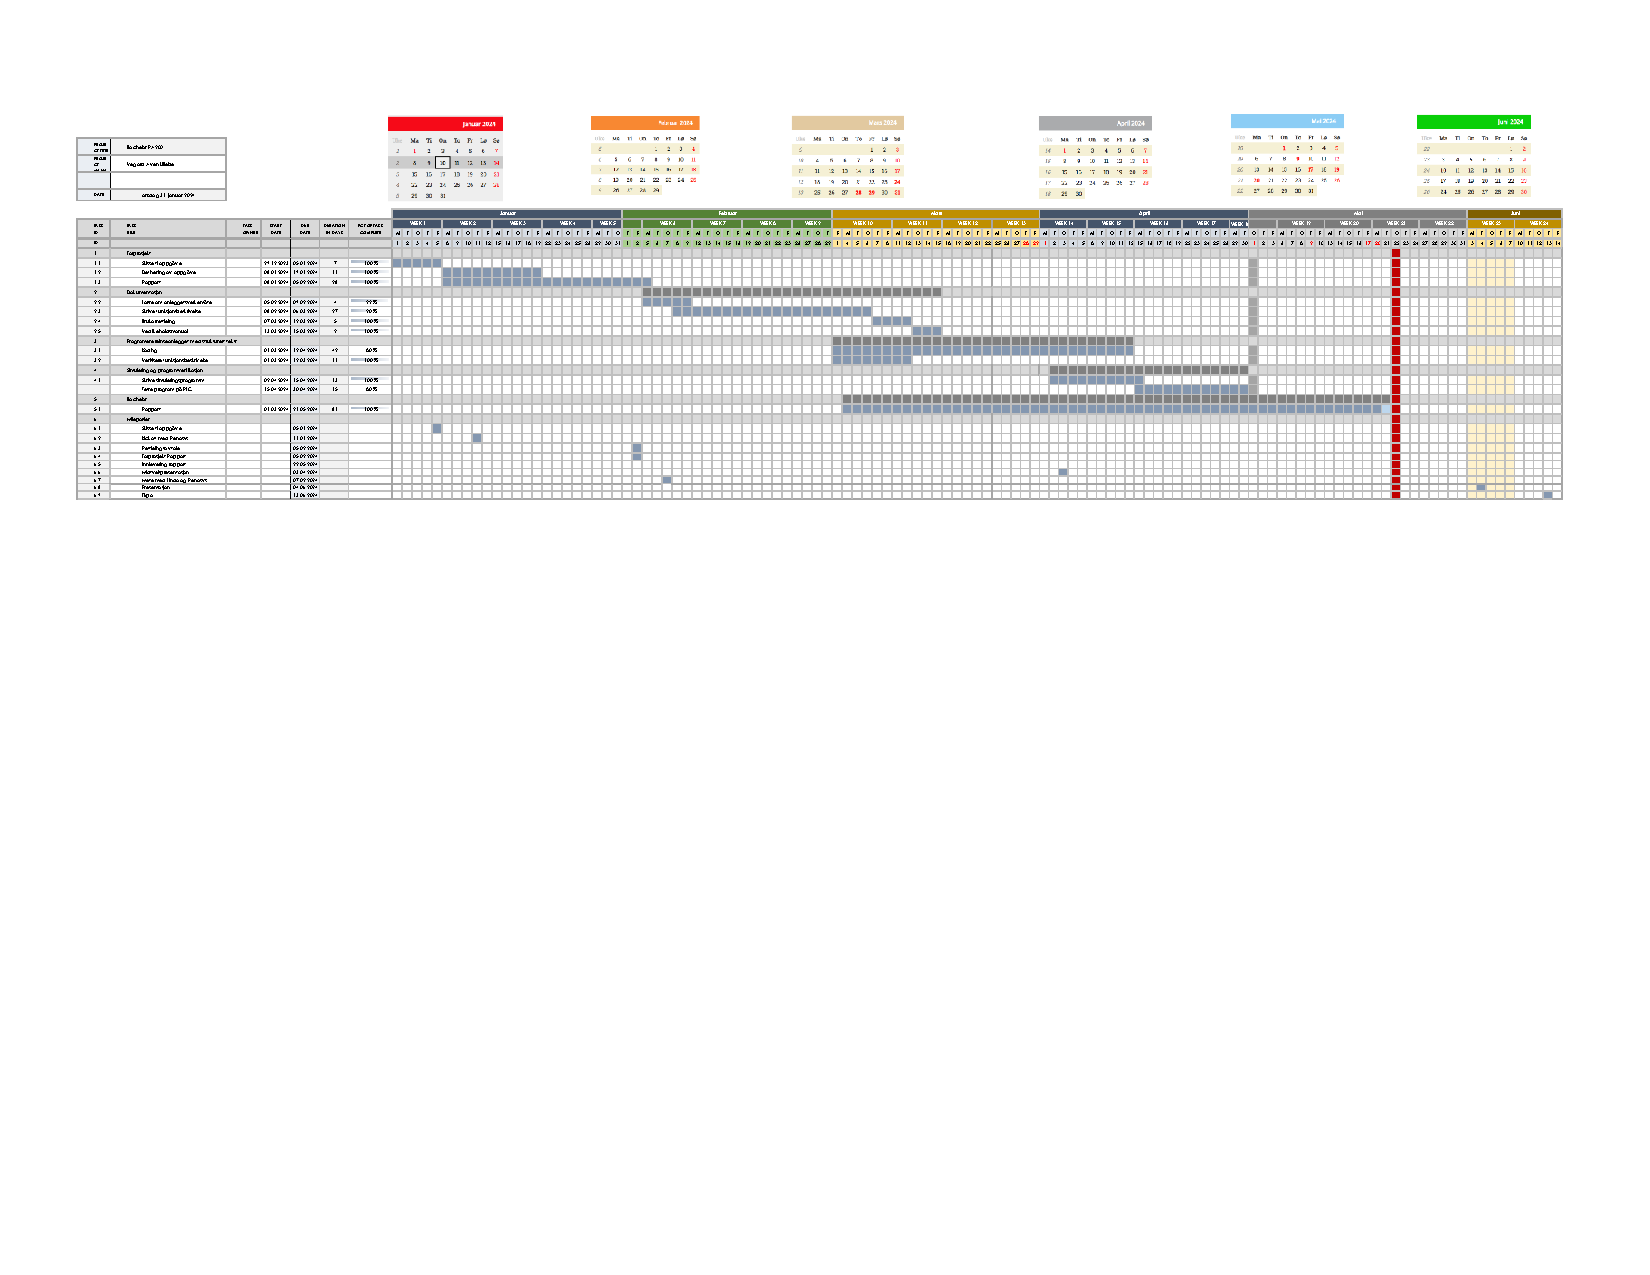
\includepdf[pages=1, angle=90,scale=0.8, pagecommand={\chapter{Gant}\thispagestyle{fancy}},fitpaper=true]{Vedlegg/Gant2.pdf}

% ------------ Nytt Kapittel
\chapter{Funksjons Blokker}
\thispagestyle{fancy}

% Sekvens Blokker 
% FB Pause
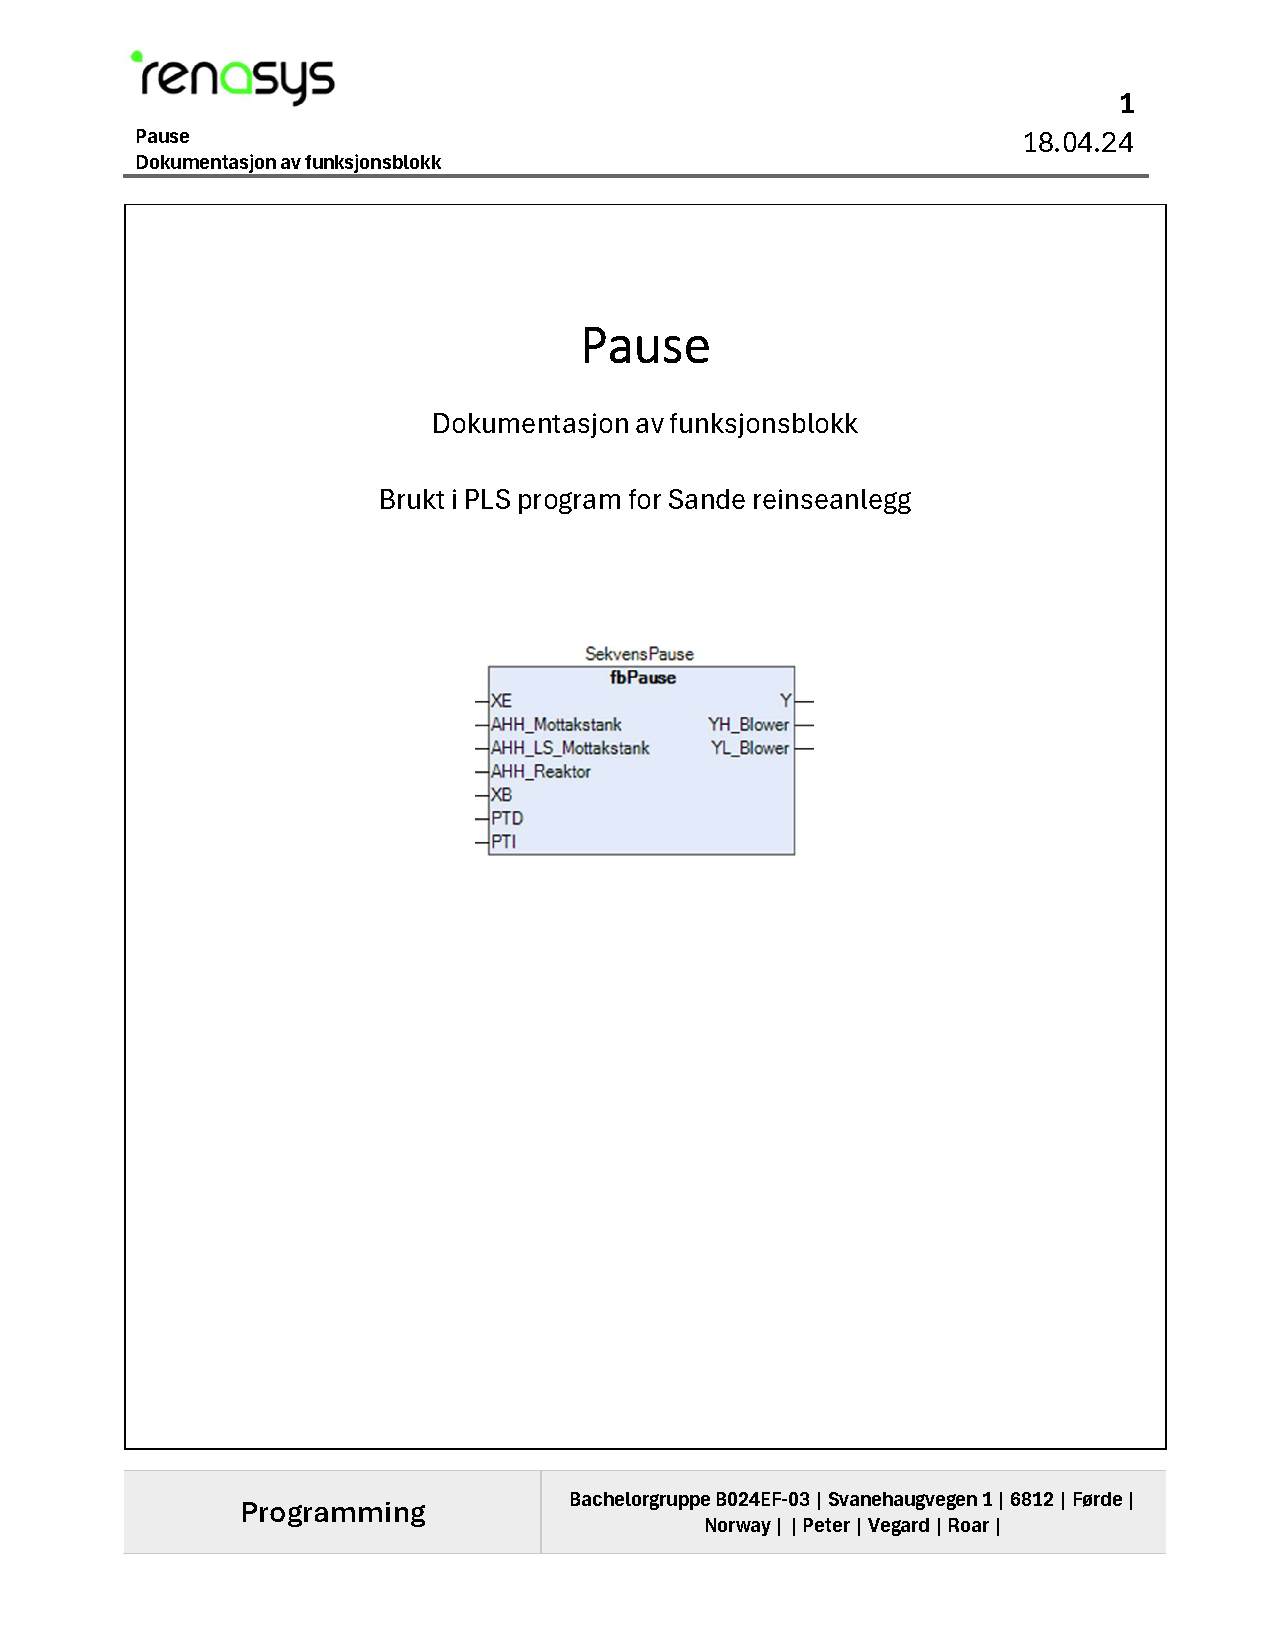
\includepdf[pages=1, scale=0.8, pagecommand={\section{FB Pause Sekvens}\thispagestyle{fancy}}, fitpaper=true ]{Vedlegg/Funksjons Blokker/fbPause.pdf}
\includepdf[pages=2-,scale=0.8, pagecommand={\thispagestyle{fancy}},fitpaper=true]{Vedlegg/Funksjons Blokker/fbPause.pdf}
% FB Innpumping
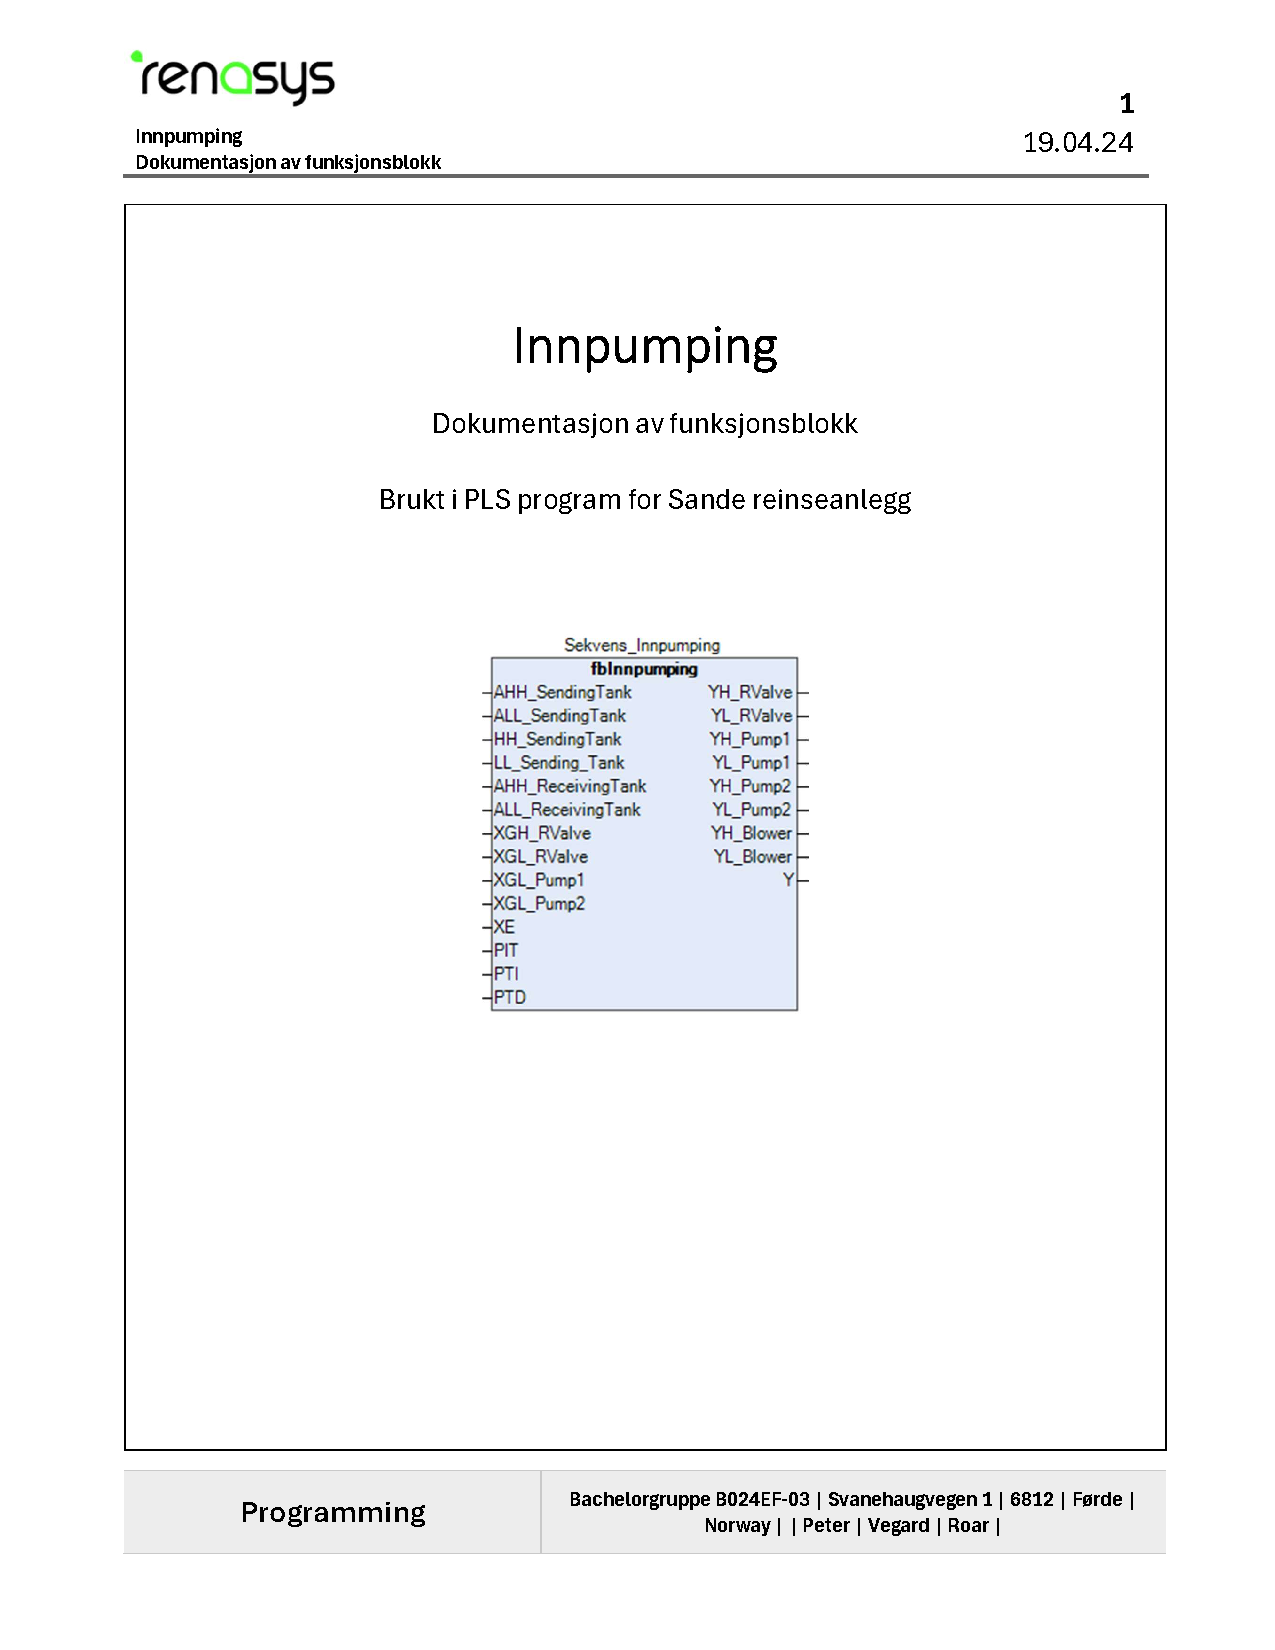
\includepdf[pages=1, scale=0.8, pagecommand={\section{FB Innpumpings Sekvens}\thispagestyle{fancy}}, fitpaper=true ]{Vedlegg/Funksjons Blokker/fbInnpumping.pdf}
\includepdf[pages=2-,scale=0.8, pagecommand={\thispagestyle{fancy}},fitpaper=true]{Vedlegg/Funksjons Blokker/fbInnpumping.pdf}
% FB Reaksjon
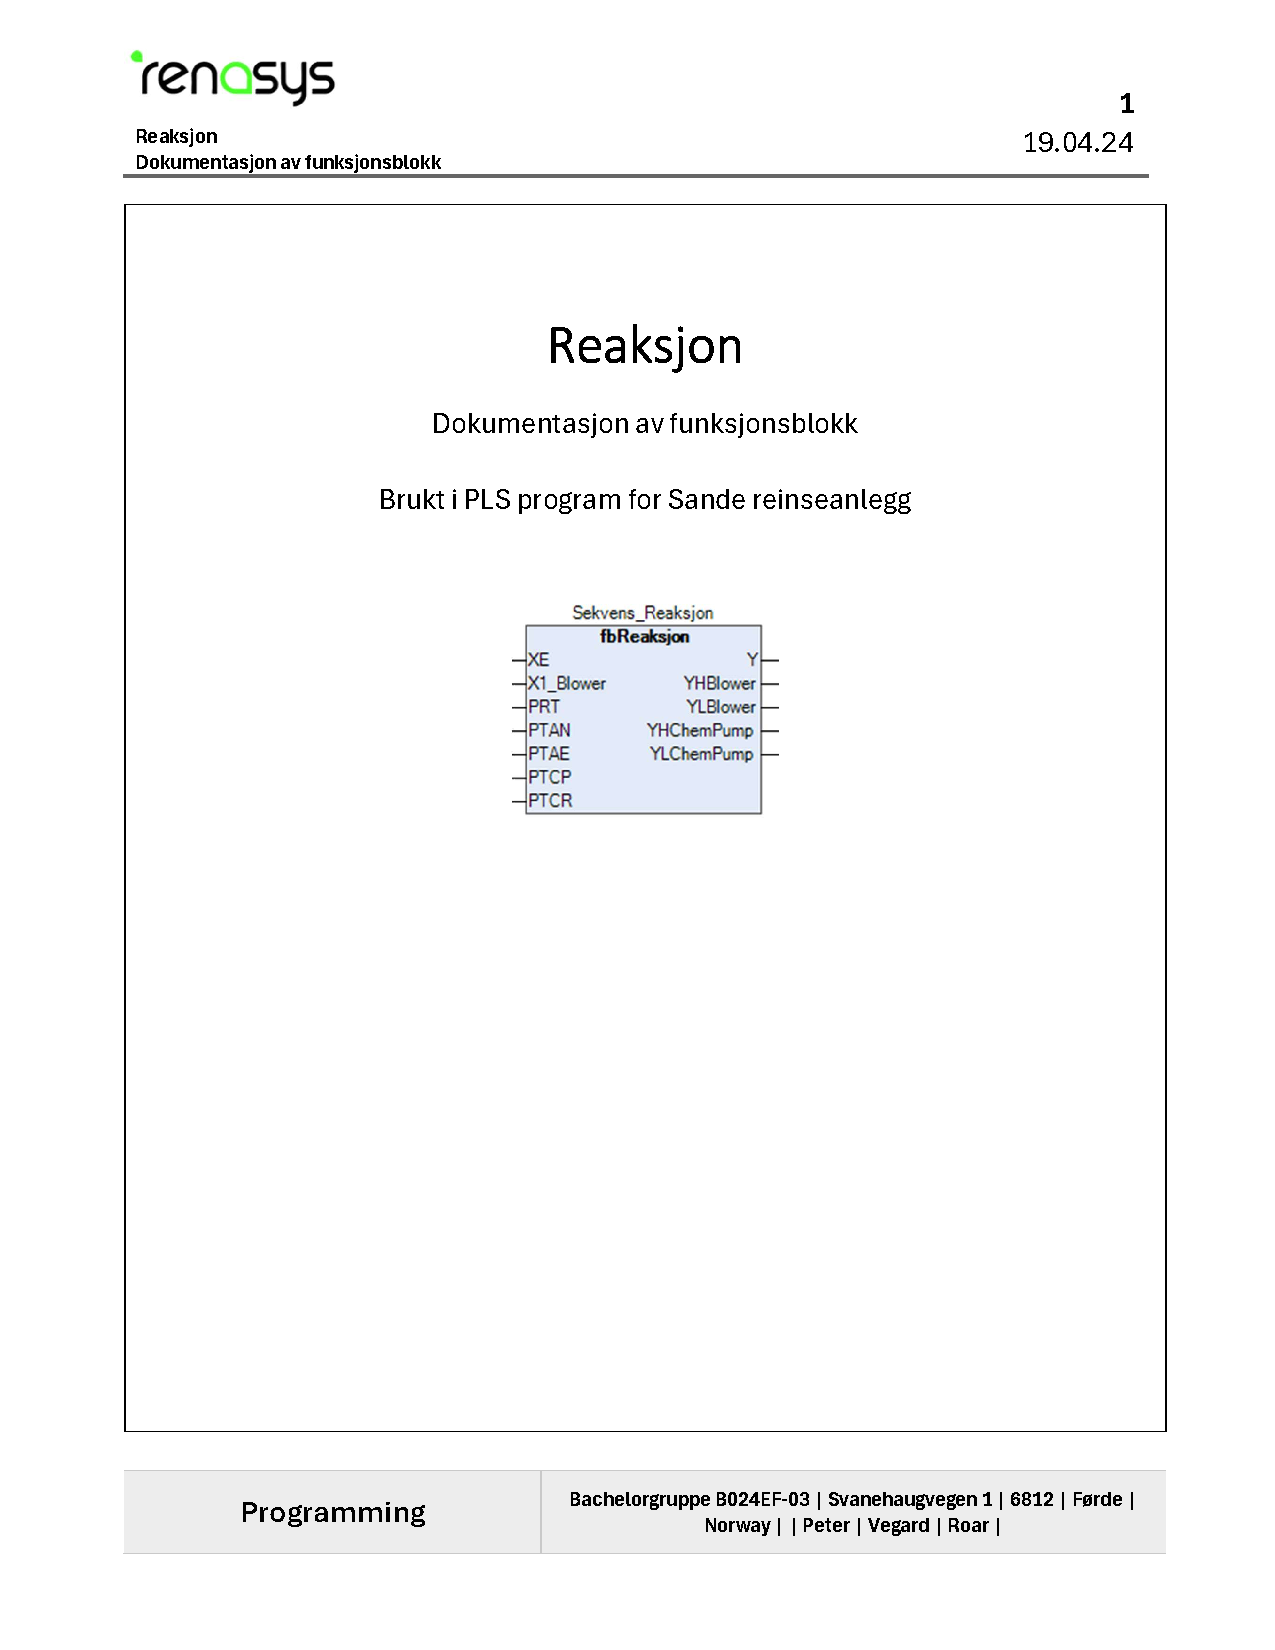
\includepdf[pages=1, scale=0.8, pagecommand={\section{FB Reaksjon Sekvens}\thispagestyle{fancy}}, fitpaper=true ]{Vedlegg/Funksjons Blokker/fbReaksjon Dokumentasjon.pdf}
\includepdf[pages=2-,scale=0.8, pagecommand={\thispagestyle{fancy}},fitpaper=true]{Vedlegg/Funksjons Blokker/fbReaksjon Dokumentasjon.pdf}
% FB Sedimentering
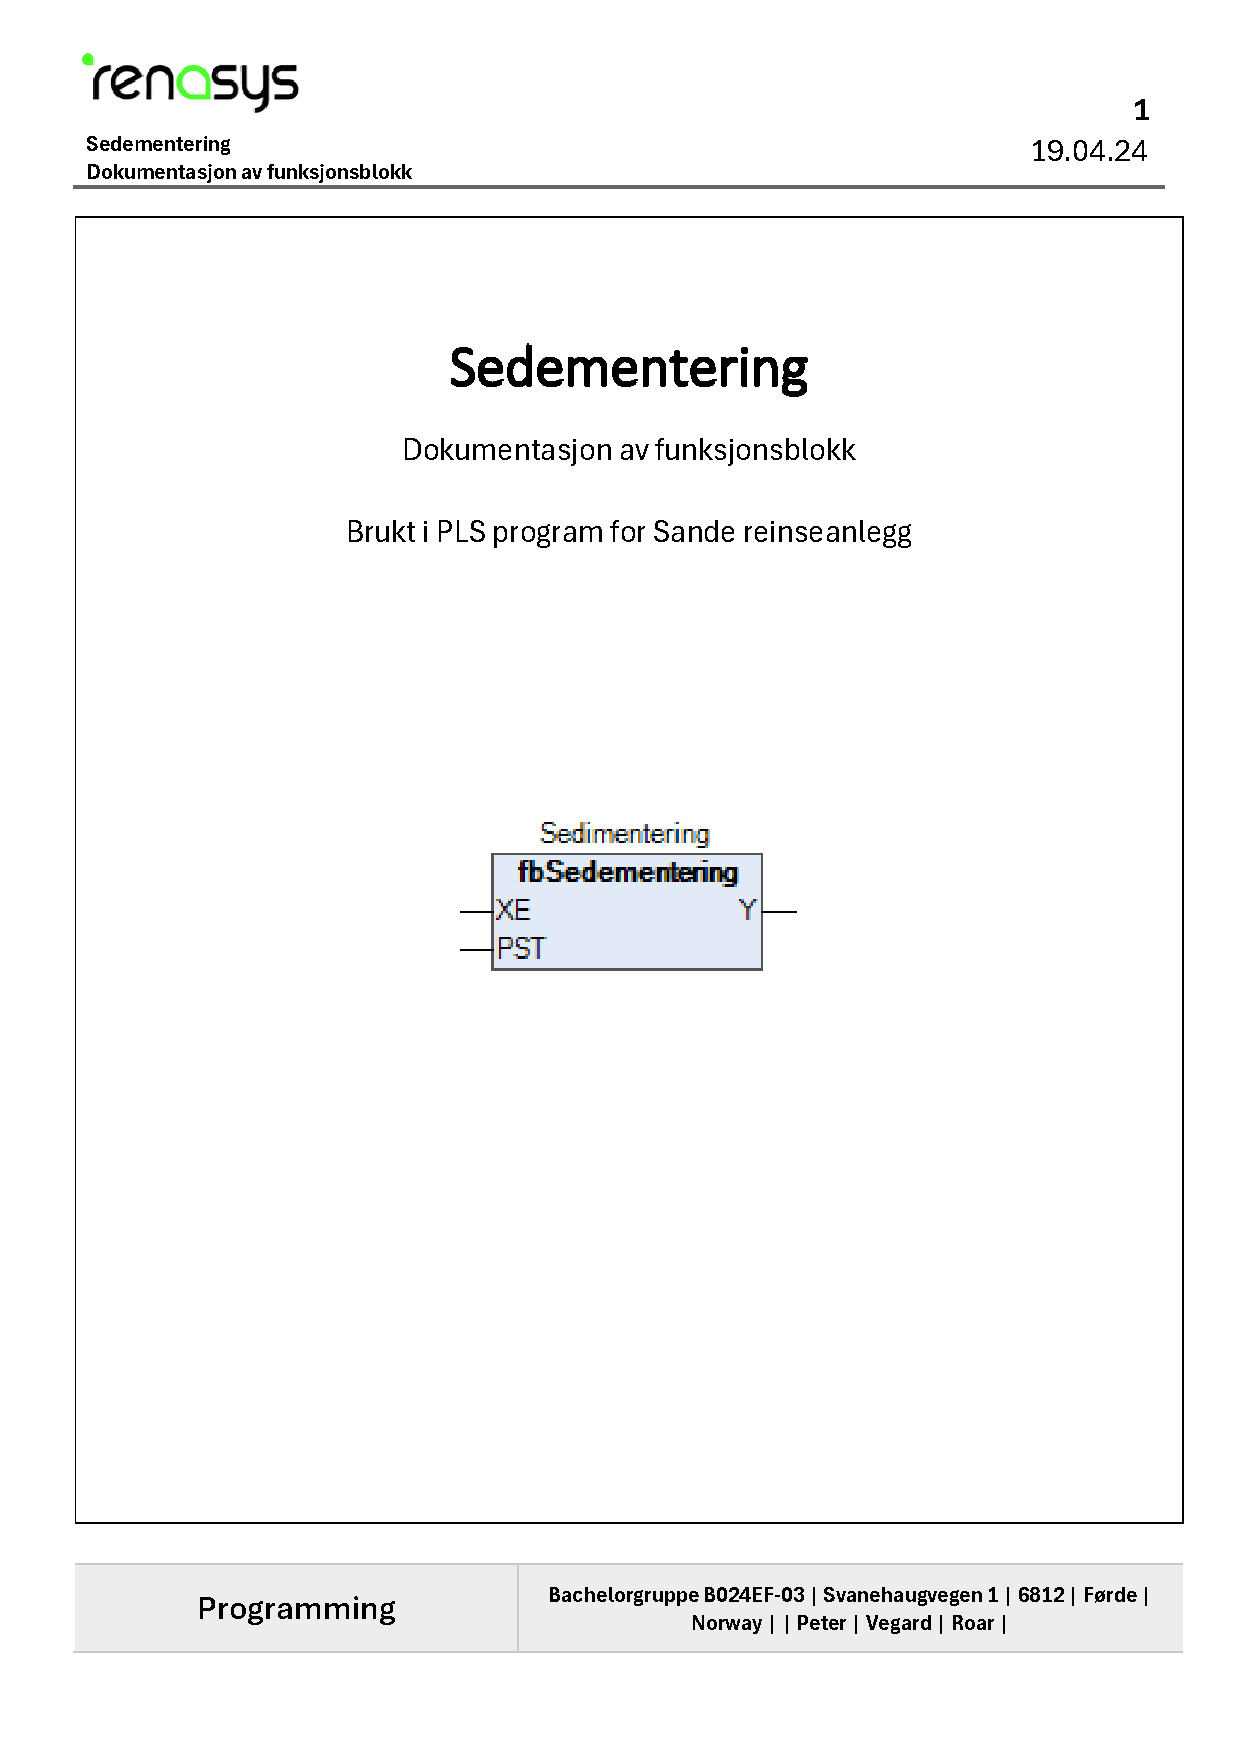
\includepdf[pages=1, scale=0.8, pagecommand={\section{FB Sedimentering Sekvens}\thispagestyle{fancy}}, fitpaper=true ]{Vedlegg/Funksjons Blokker/fbSedementering Dokumentasjon.pdf}
\includepdf[pages=2-,scale=0.8, pagecommand={\thispagestyle{fancy}},fitpaper=true]{Vedlegg/Funksjons Blokker/fbSedementering Dokumentasjon.pdf}
% FB Uttapping
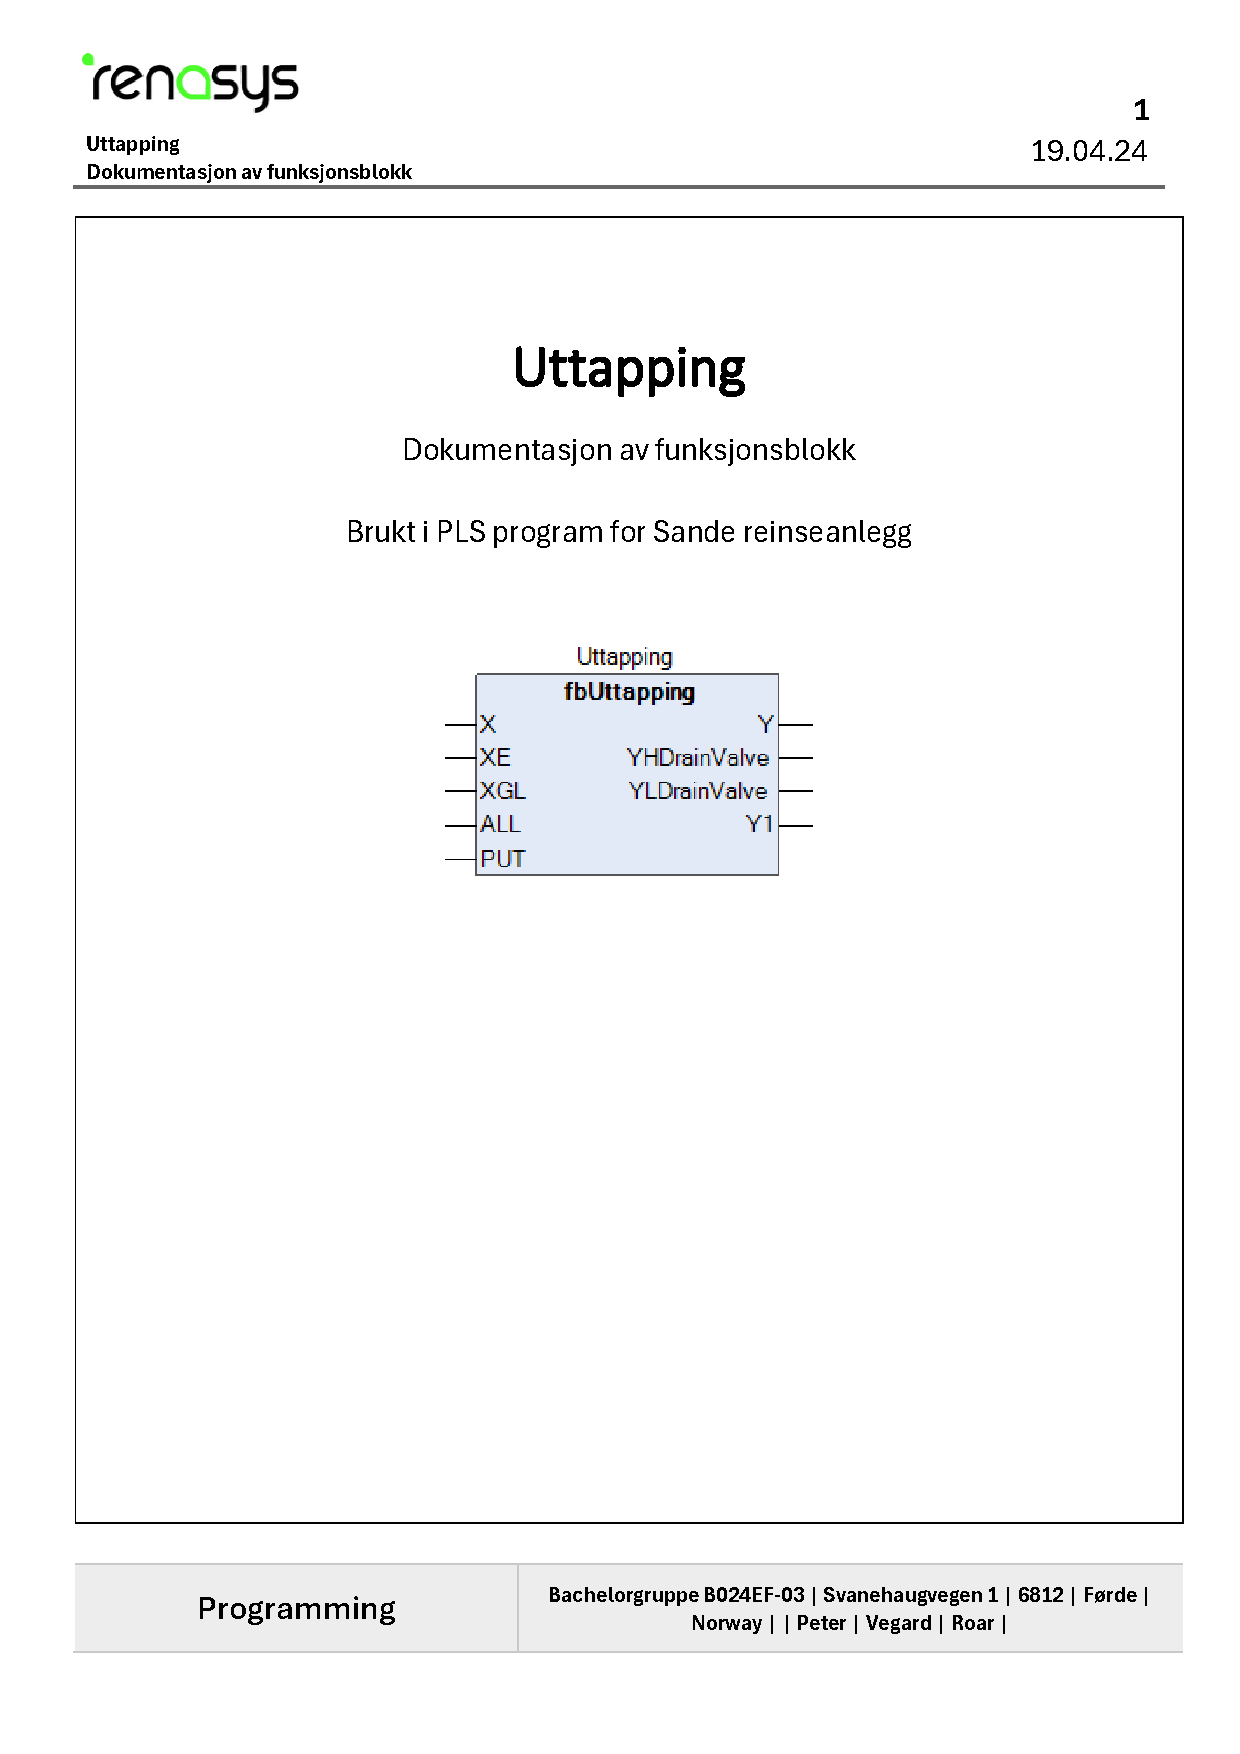
\includepdf[pages=1, scale=0.8, pagecommand={\section{FB Uttapping Sekvens}\thispagestyle{fancy}}, fitpaper=true ]{Vedlegg/Funksjons Blokker/fbUttaping Dokumentasjon.pdf}
\includepdf[pages=2-,scale=0.8, pagecommand={\thispagestyle{fancy}},fitpaper=true]{Vedlegg/Funksjons Blokker/fbUttaping Dokumentasjon.pdf}
% FB Slammuttak
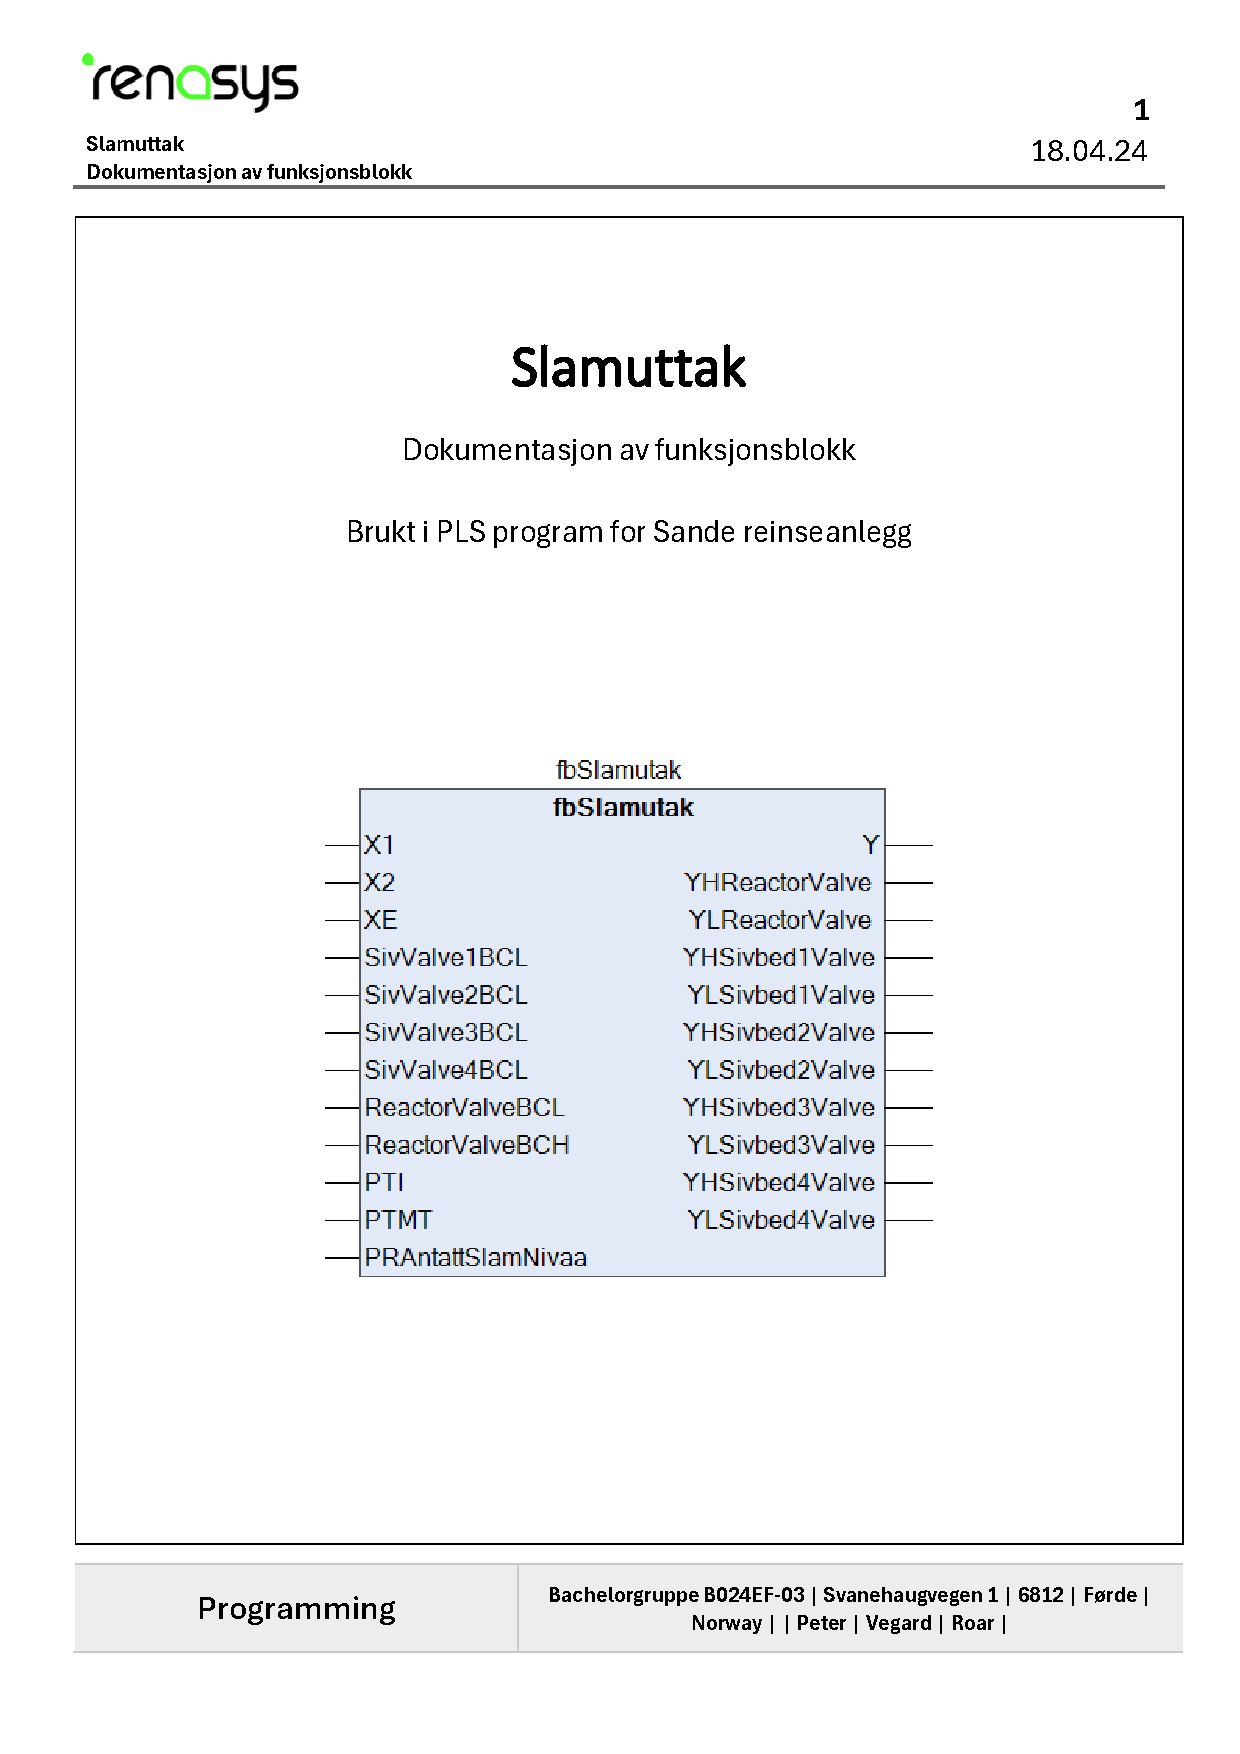
\includepdf[pages=1, scale=0.8, pagecommand={\section{FB Slammuttak}\thispagestyle{fancy}}, fitpaper=true ]{Vedlegg/Funksjons Blokker/fbSlamuttak Dokumentasjon.pdf}
\includepdf[pages=2-,scale=0.8, pagecommand={\thispagestyle{fancy}},fitpaper=true]{Vedlegg/Funksjons Blokker/fbSlamuttak Dokumentasjon.pdf}
% 
% Analog Alarm
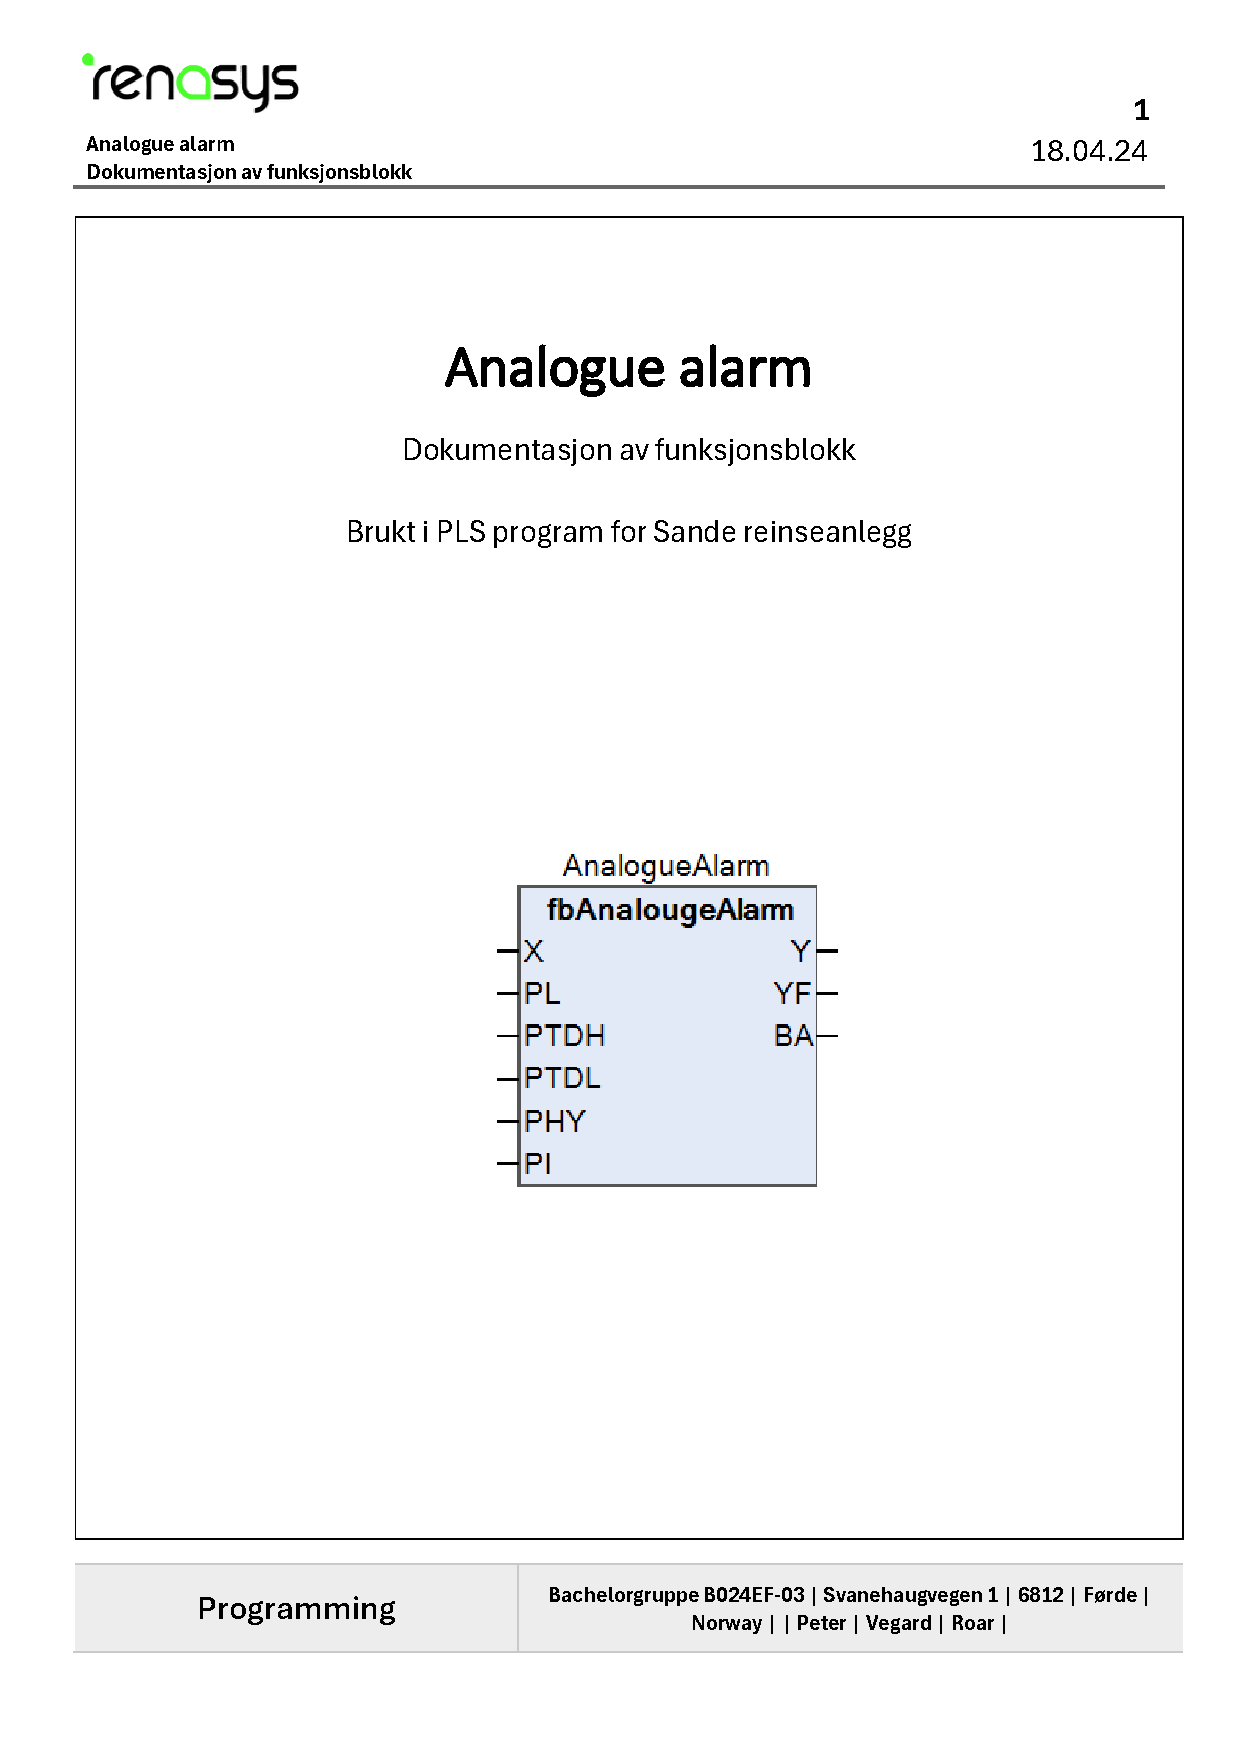
\includepdf[pages=1, scale=0.8, pagecommand={\section{FB Analog alarm}\thispagestyle{fancy}}, fitpaper=true ]{Vedlegg/Funksjons Blokker/fbAnalogueAlarm Dokumentasjon.pdf}
\includepdf[pages=2-,scale=0.8, pagecommand={\thispagestyle{fancy}},fitpaper=true]{Vedlegg/Funksjons Blokker/fbAnalogueAlarm Dokumentasjon.pdf}
% Digital Alarm
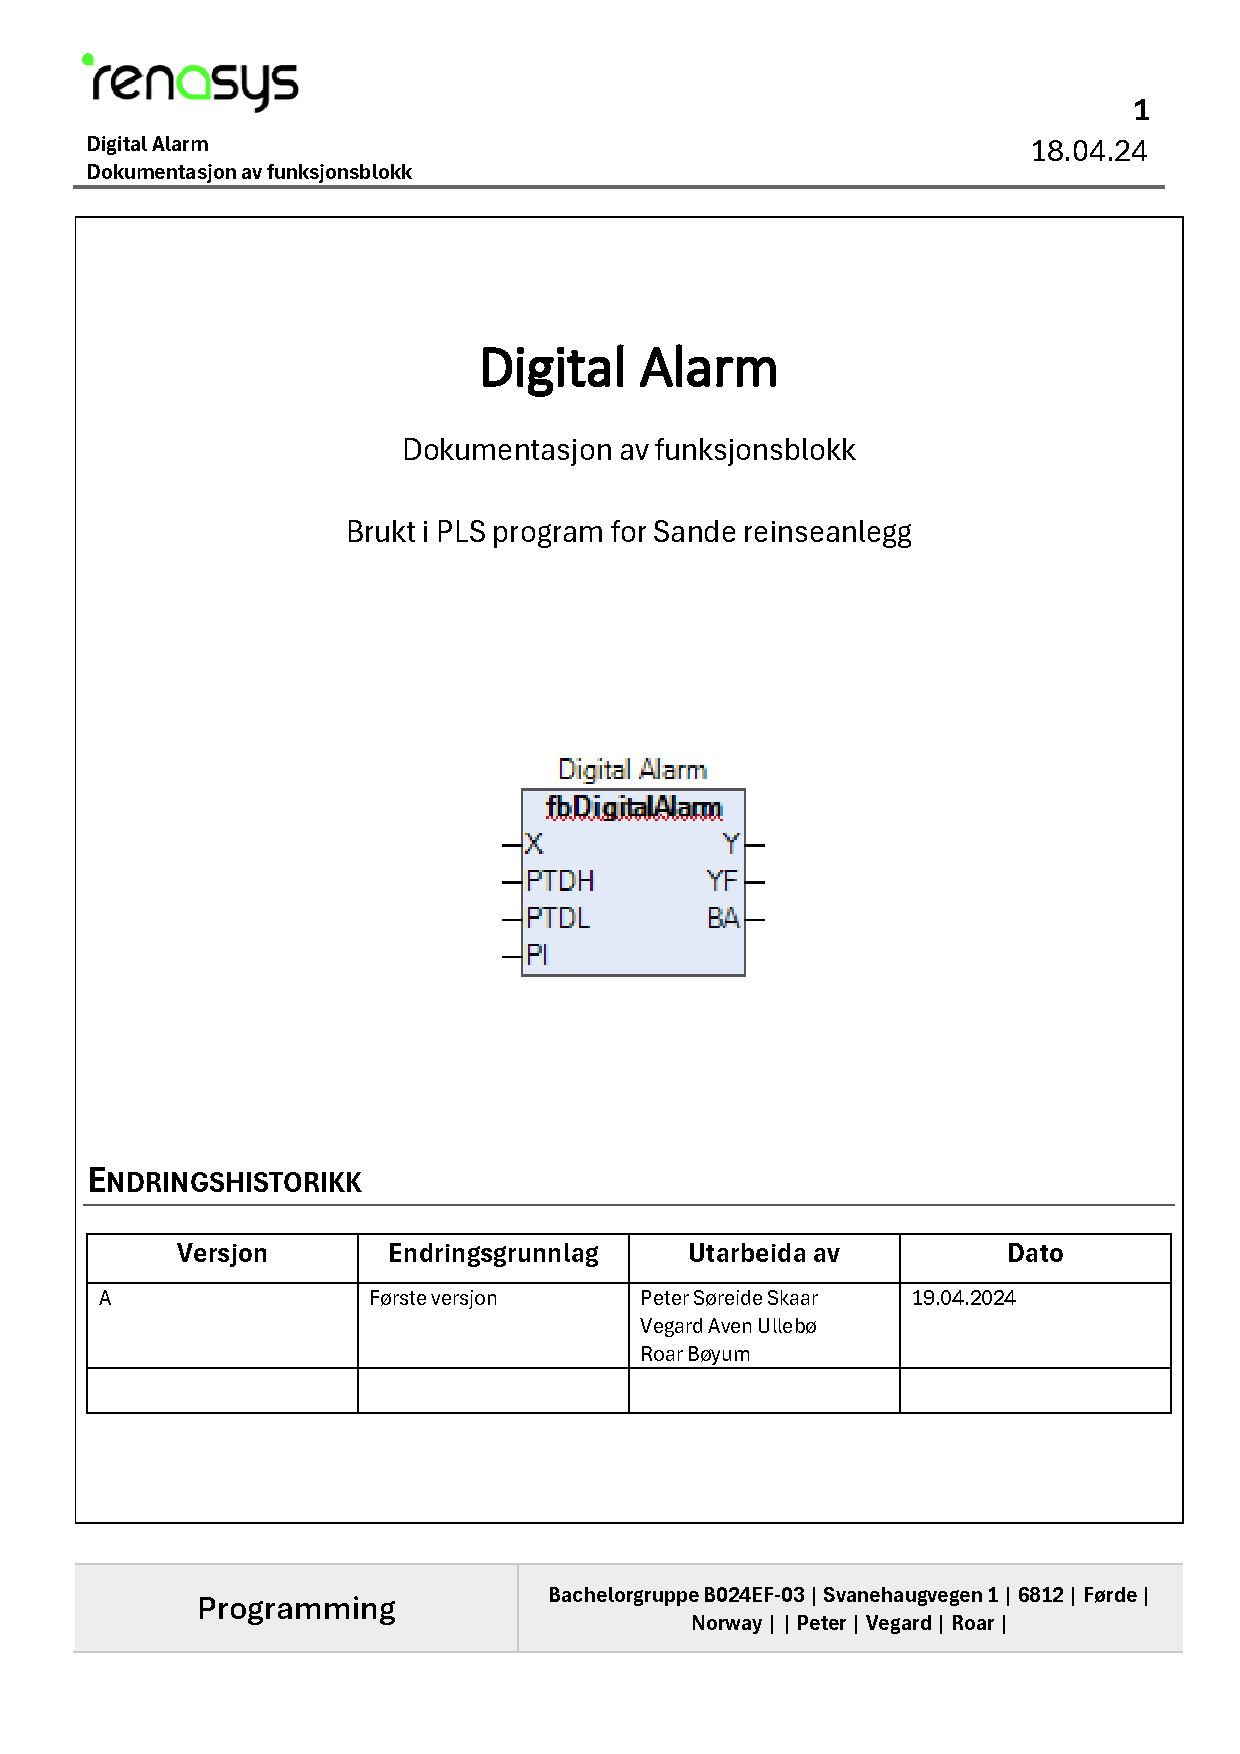
\includepdf[pages=1, scale=0.8, pagecommand={\section{FB Digital alarm}\thispagestyle{fancy}}, fitpaper=true ]{Vedlegg/Funksjons Blokker/fbDigitalAlarm.pdf}
\includepdf[pages=2-,scale=0.8, pagecommand={\thispagestyle{fancy}},fitpaper=true]{Vedlegg/Funksjons Blokker/fbDigitalAlarm.pdf}
% Calculations

\includepdf[pages=1, scale=0.8, pagecommand={\section{FB Kalkuleringer}\thispagestyle{fancy}}, fitpaper=true ]{Vedlegg/Funksjons Blokker/fbCalculations.pdf}

\includepdf[pages=2-,scale=0.8, pagecommand={\thispagestyle{fancy}},fitpaper=true]{Vedlegg/Funksjons Blokker/fbCalculations.pdf}
% Data Processing
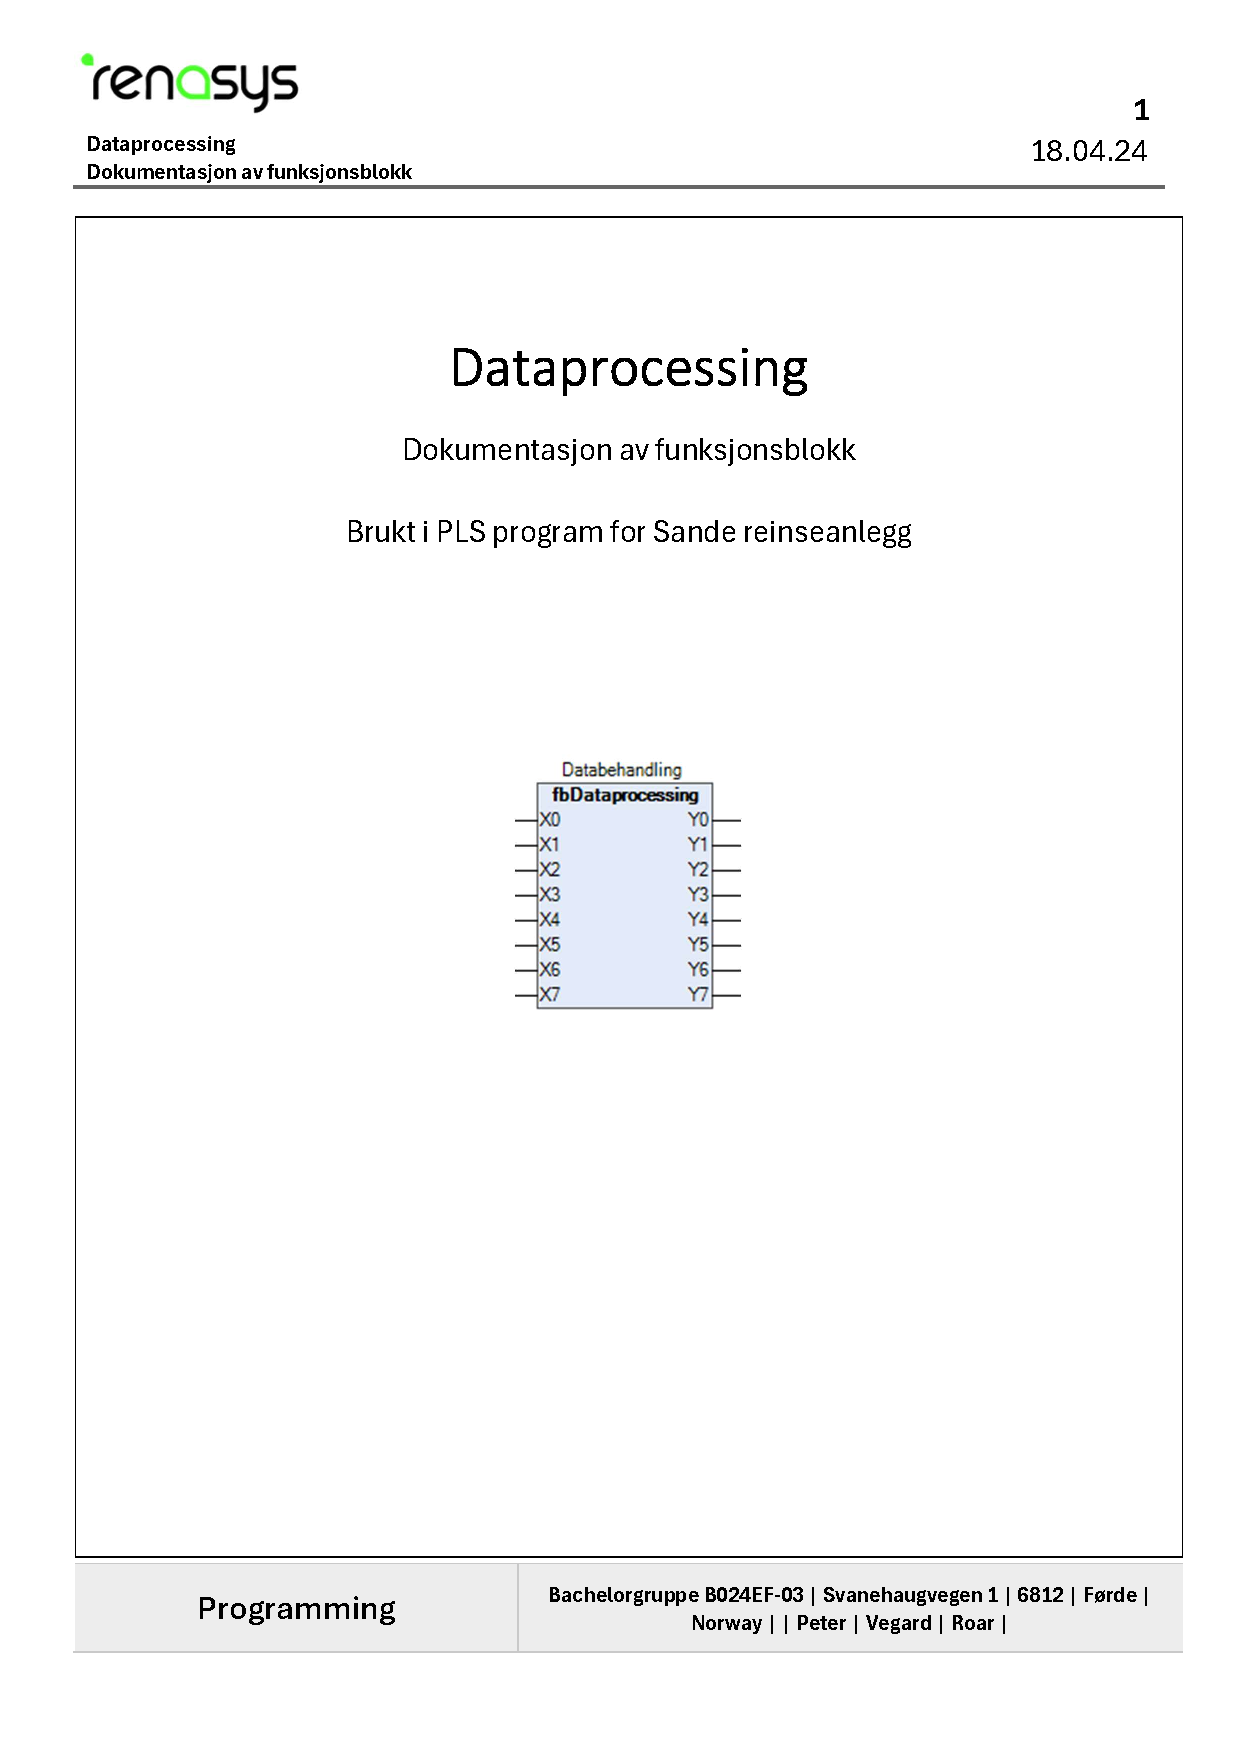
\includepdf[pages=1, scale=0.8, pagecommand={\section{FB Data Prossesering}\thispagestyle{fancy}}, fitpaper=true ]{Vedlegg/Funksjons Blokker/fbDataProcessing.pdf}
\includepdf[pages=2-,scale=0.8, pagecommand={\thispagestyle{fancy}},fitpaper=true]{Vedlegg/Funksjons Blokker/fbDataProcessing.pdf}
% Høgbelastningsmodus
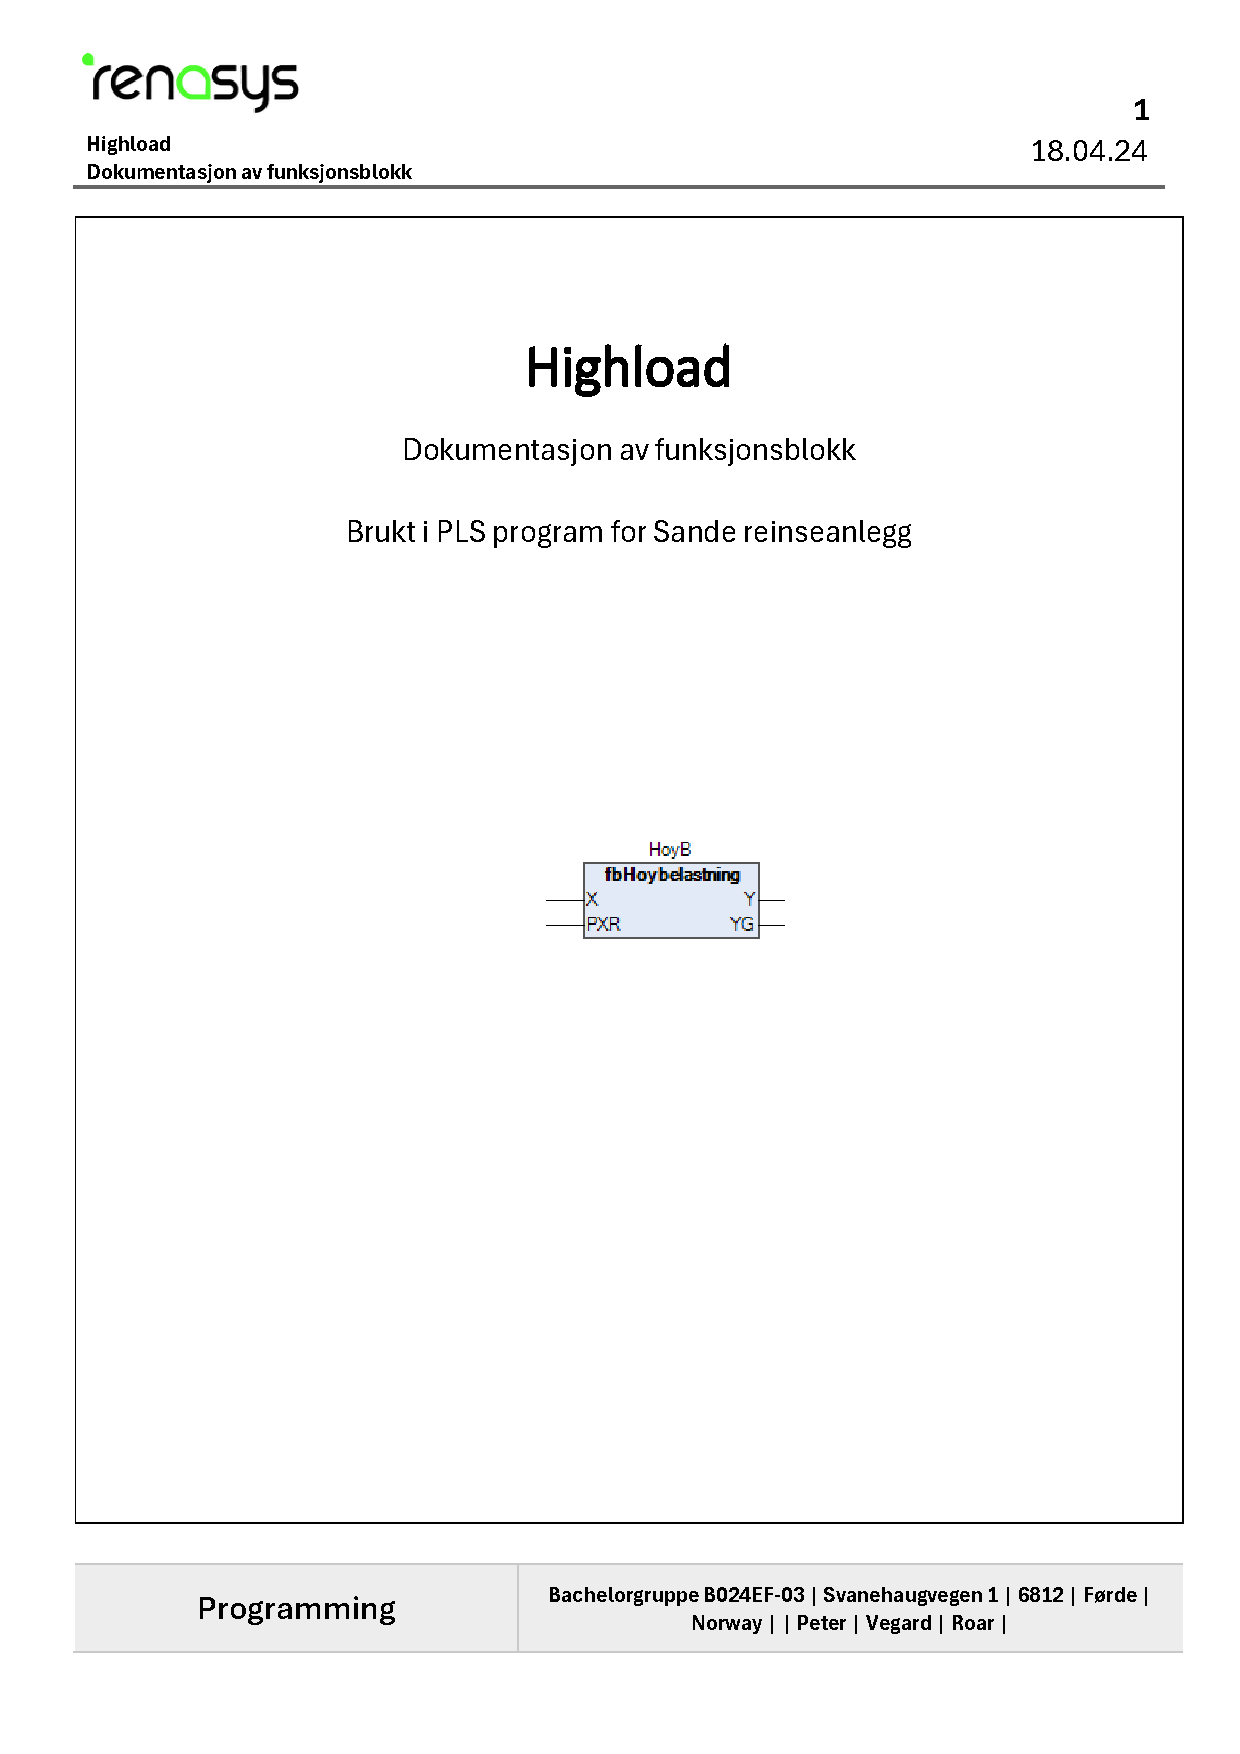
\includepdf[pages=1, scale=0.8, pagecommand={\section{FB High Load}\thispagestyle{fancy}}, fitpaper=true ]{Vedlegg/Funksjons Blokker/fbHighLoad.pdf}
\includepdf[pages=2-,scale=0.8, pagecommand={\thispagestyle{fancy}},fitpaper=true]{Vedlegg/Funksjons Blokker/fbHighLoad.pdf}
% Processed Water
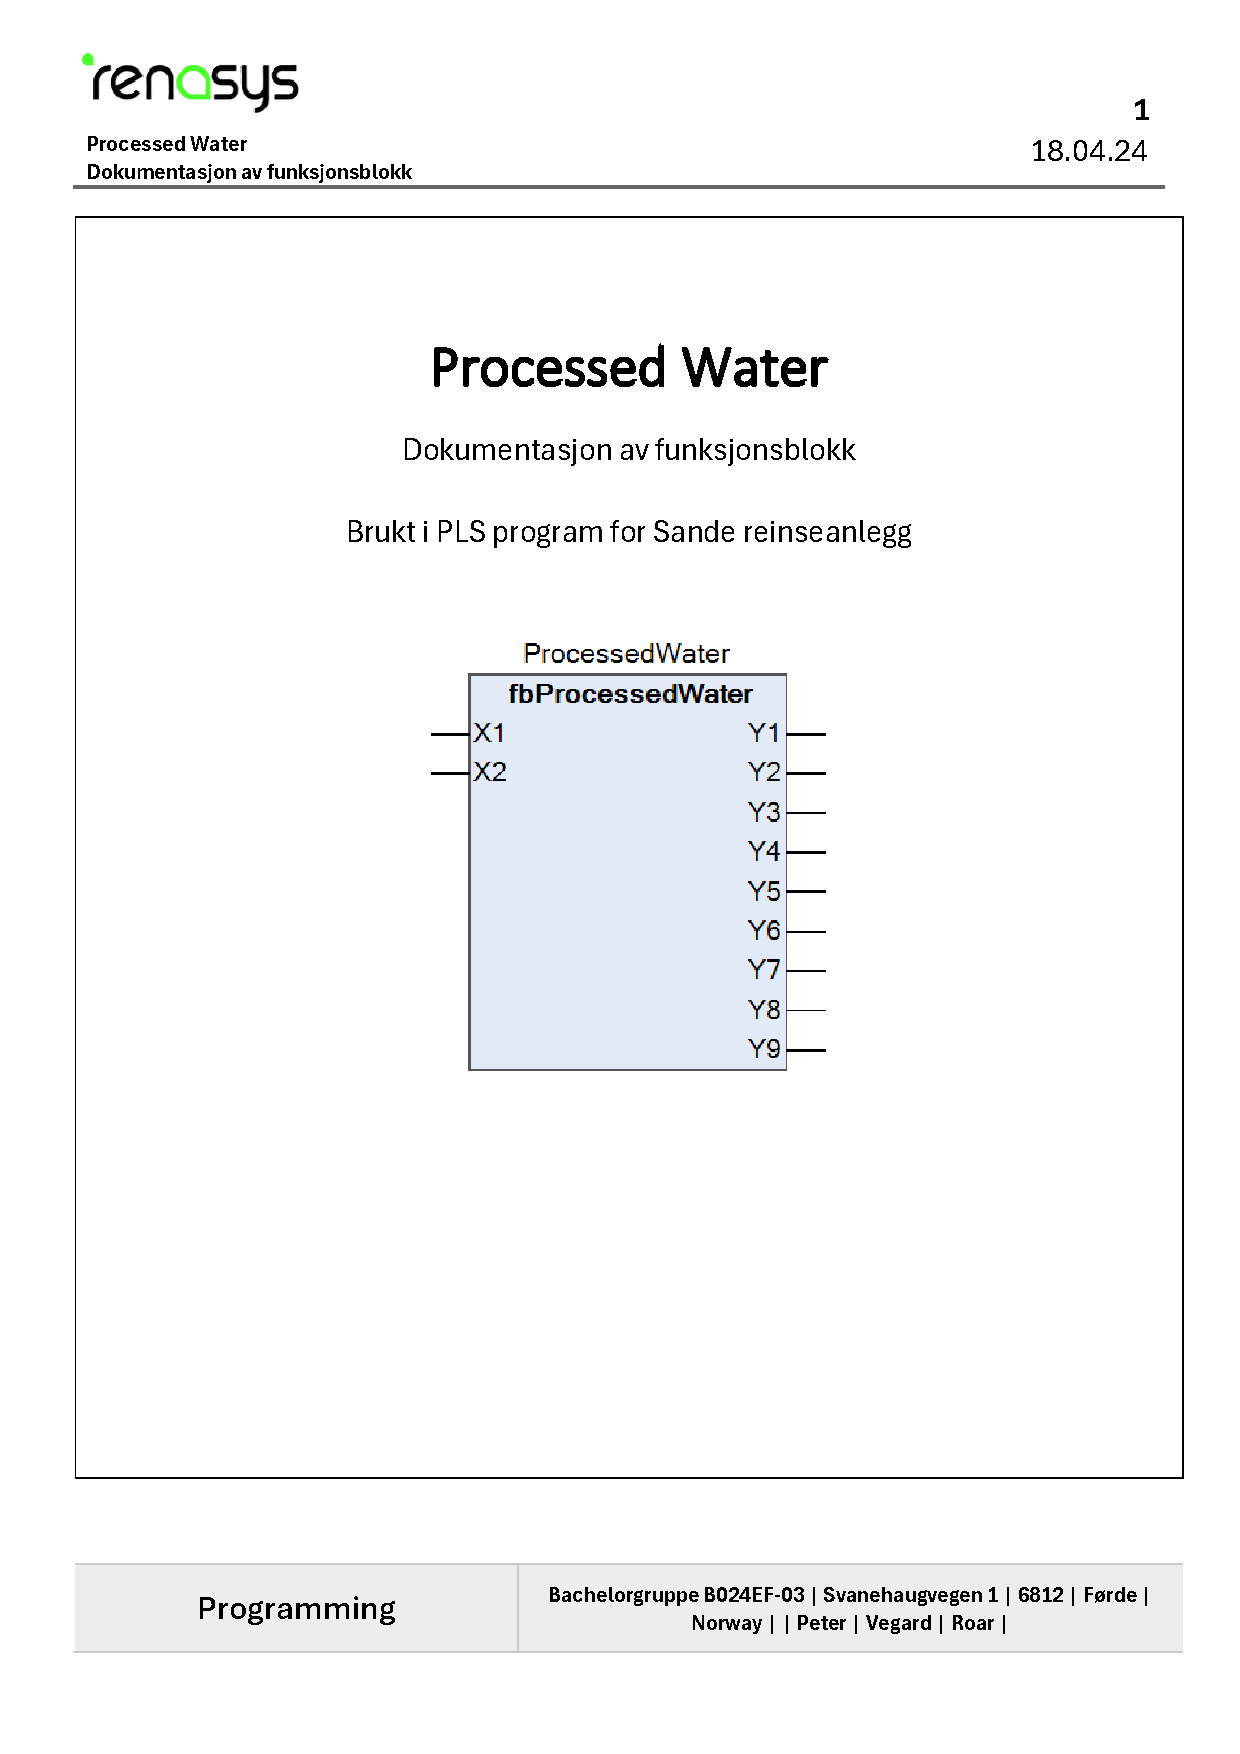
\includepdf[pages=1, scale=0.8, pagecommand={\section{FB Processed Water}\thispagestyle{fancy}}, fitpaper=true ]{Vedlegg/Funksjons Blokker/fbProcessedWater Dokumentasjon.pdf}
\includepdf[pages=2-,scale=0.8, pagecommand={\thispagestyle{fancy}},fitpaper=true]{Vedlegg/Funksjons Blokker/fbProcessedWater Dokumentasjon.pdf}
% fbPumpInterlock
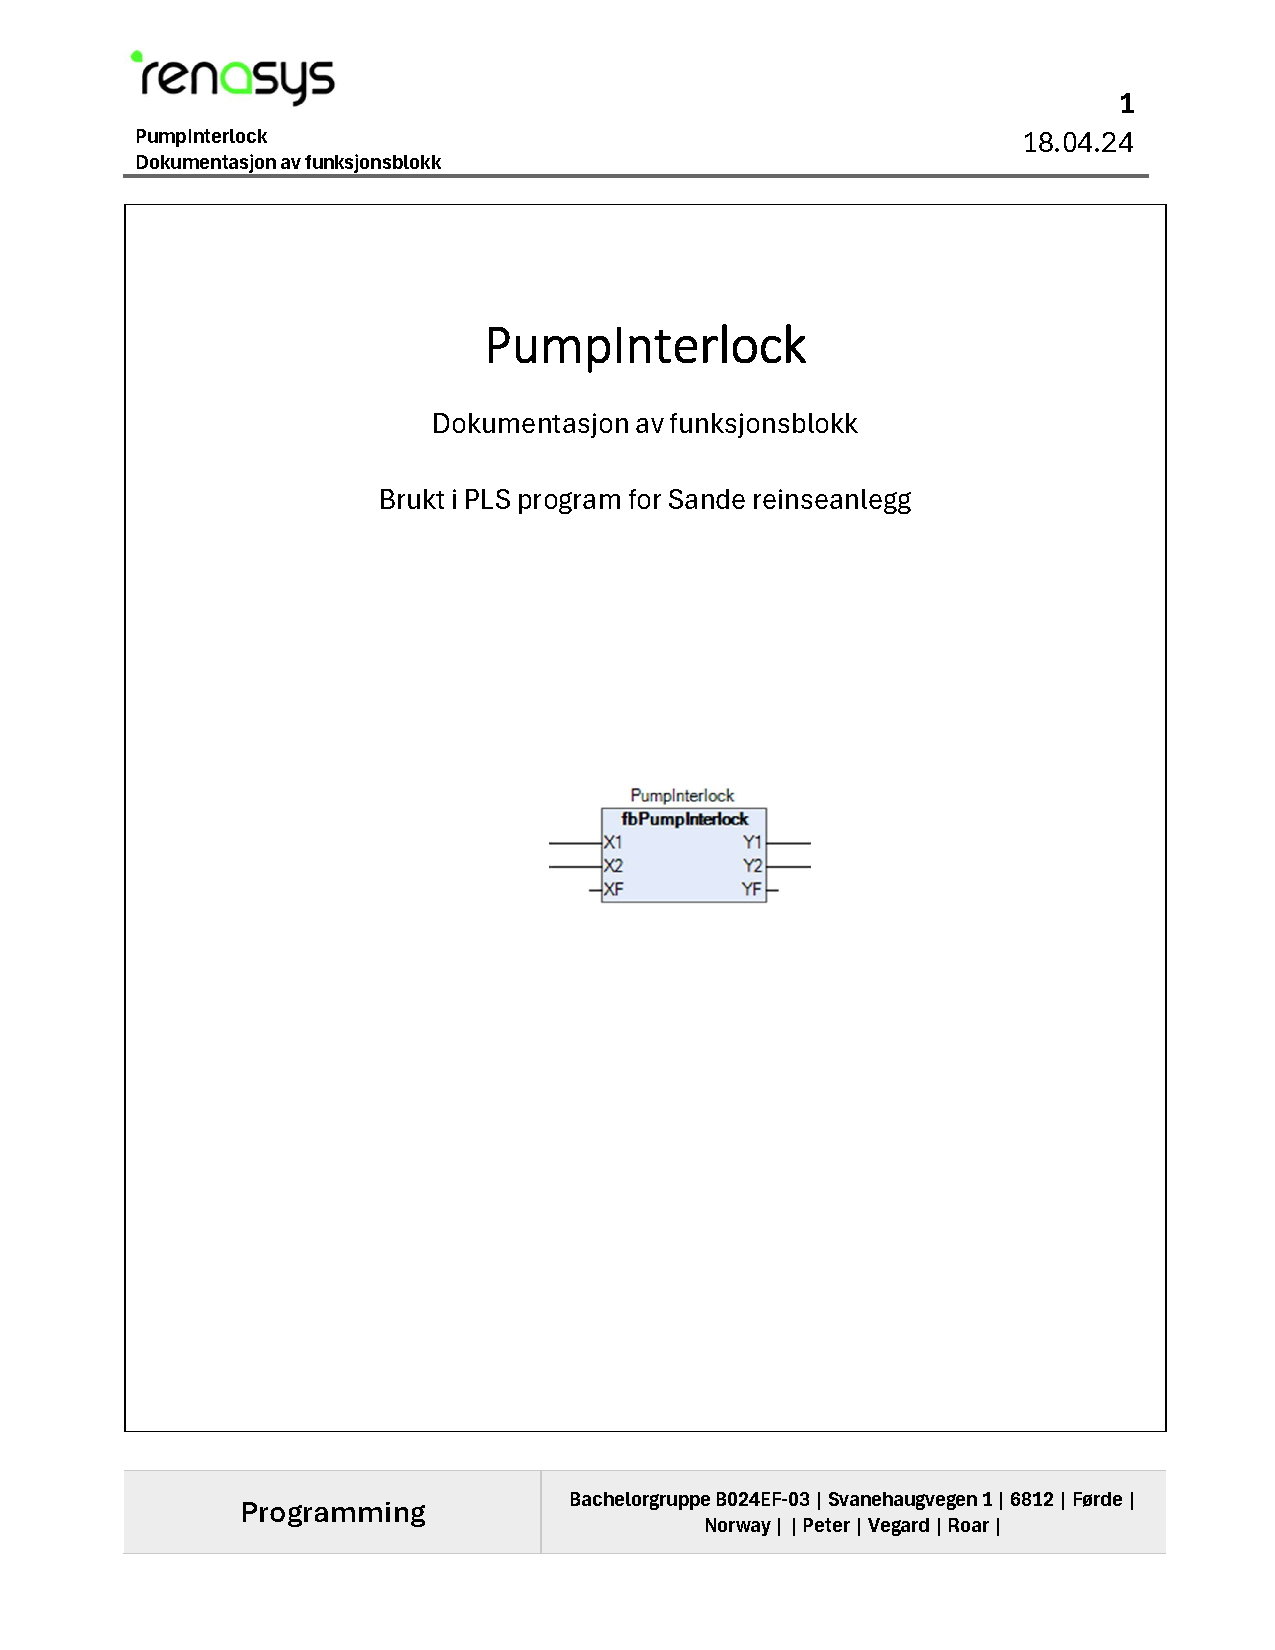
\includepdf[pages=1, scale=0.8, pagecommand={\section{FB Pump Interlock}\thispagestyle{fancy}}, fitpaper=true ]{Vedlegg/Funksjons Blokker/fbPumpInterlock.pdf}
\includepdf[pages=2-,scale=0.8, pagecommand={\thispagestyle{fancy}},fitpaper=true]{Vedlegg/Funksjons Blokker/fbPumpInterlock.pdf}
% Sivbed Rotation
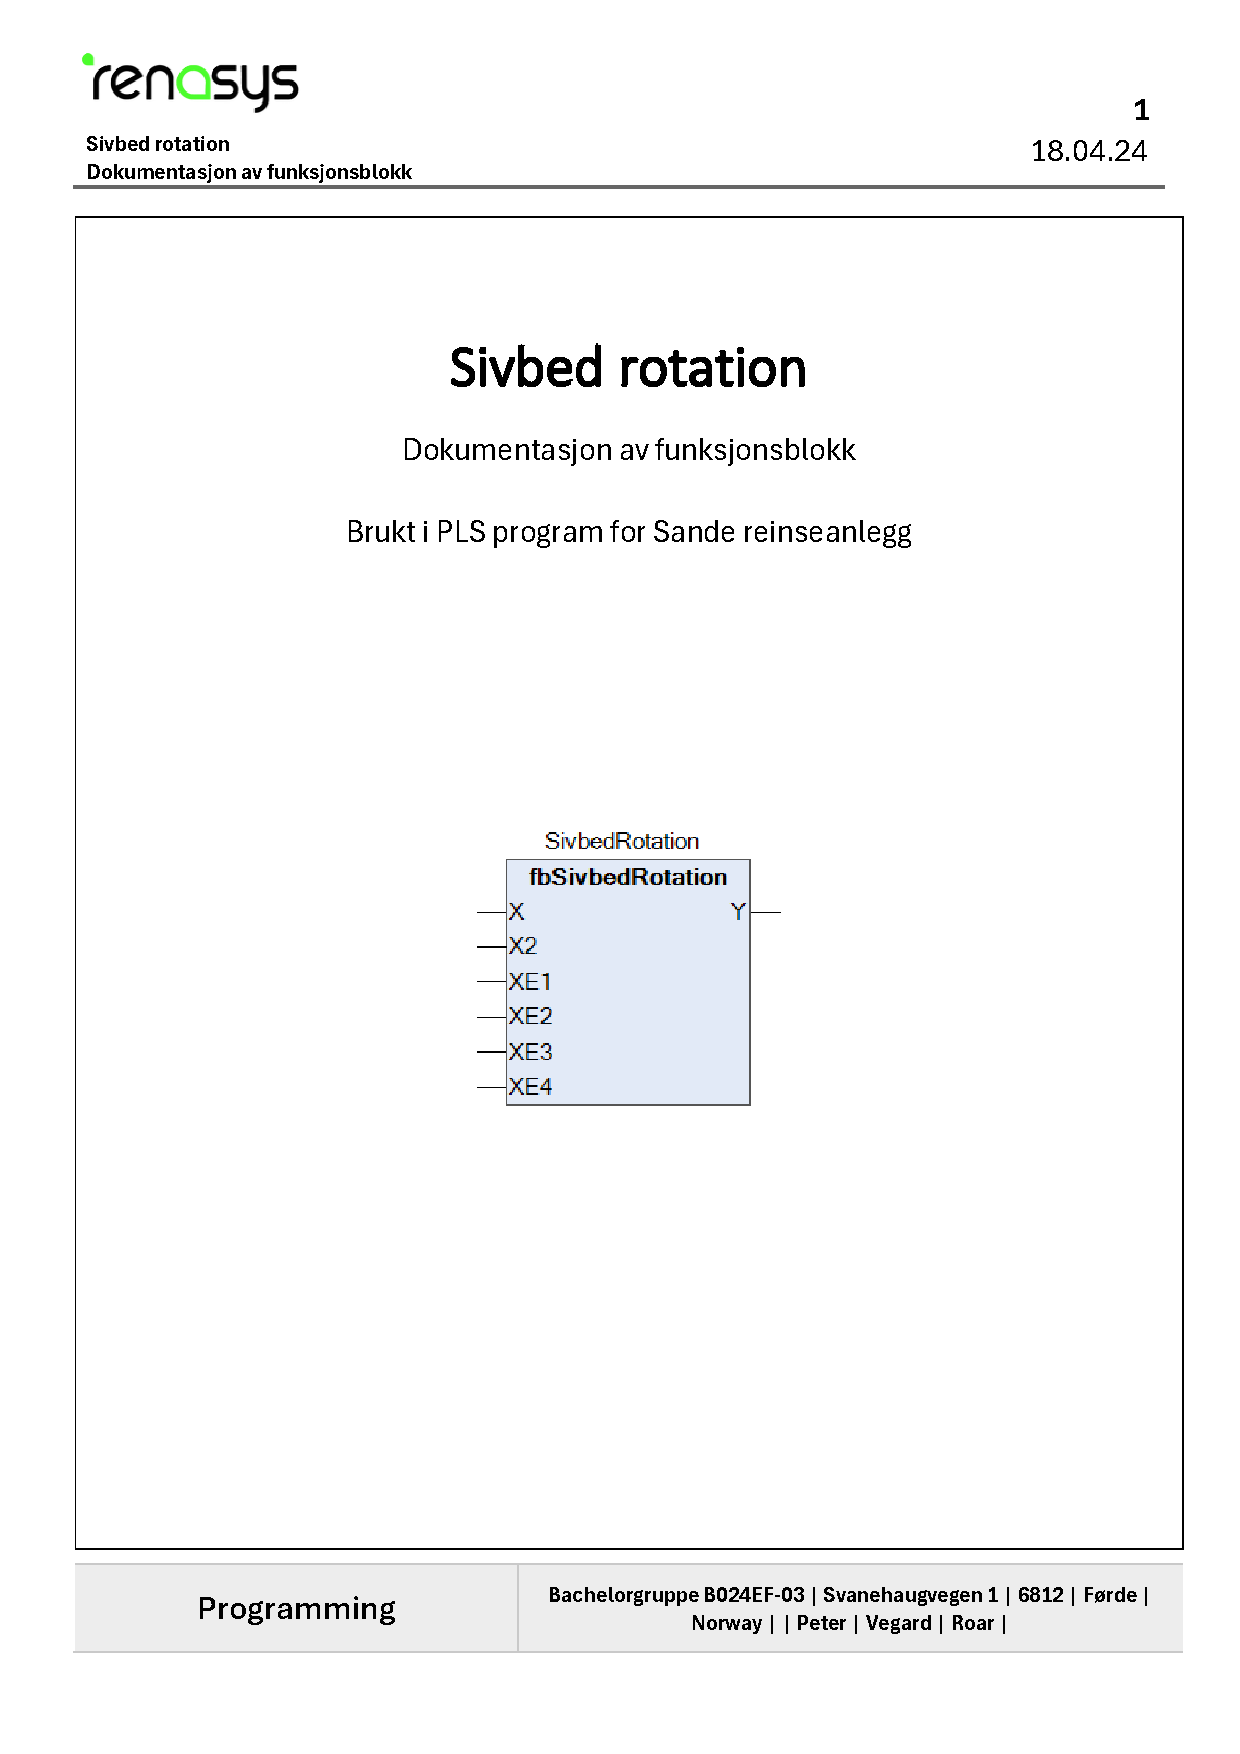
\includepdf[pages=1, scale=0.8, pagecommand={\section{FB Sivbed Rotation}\thispagestyle{fancy}}, fitpaper=true ]{Vedlegg/Funksjons Blokker/fbSivbed Rotation Dokumentasjon.pdf}
\includepdf[pages=2-,scale=0.8, pagecommand={\thispagestyle{fancy}},fitpaper=true]{Vedlegg/Funksjons Blokker/fbSivbed Rotation Dokumentasjon.pdf}
% Swap
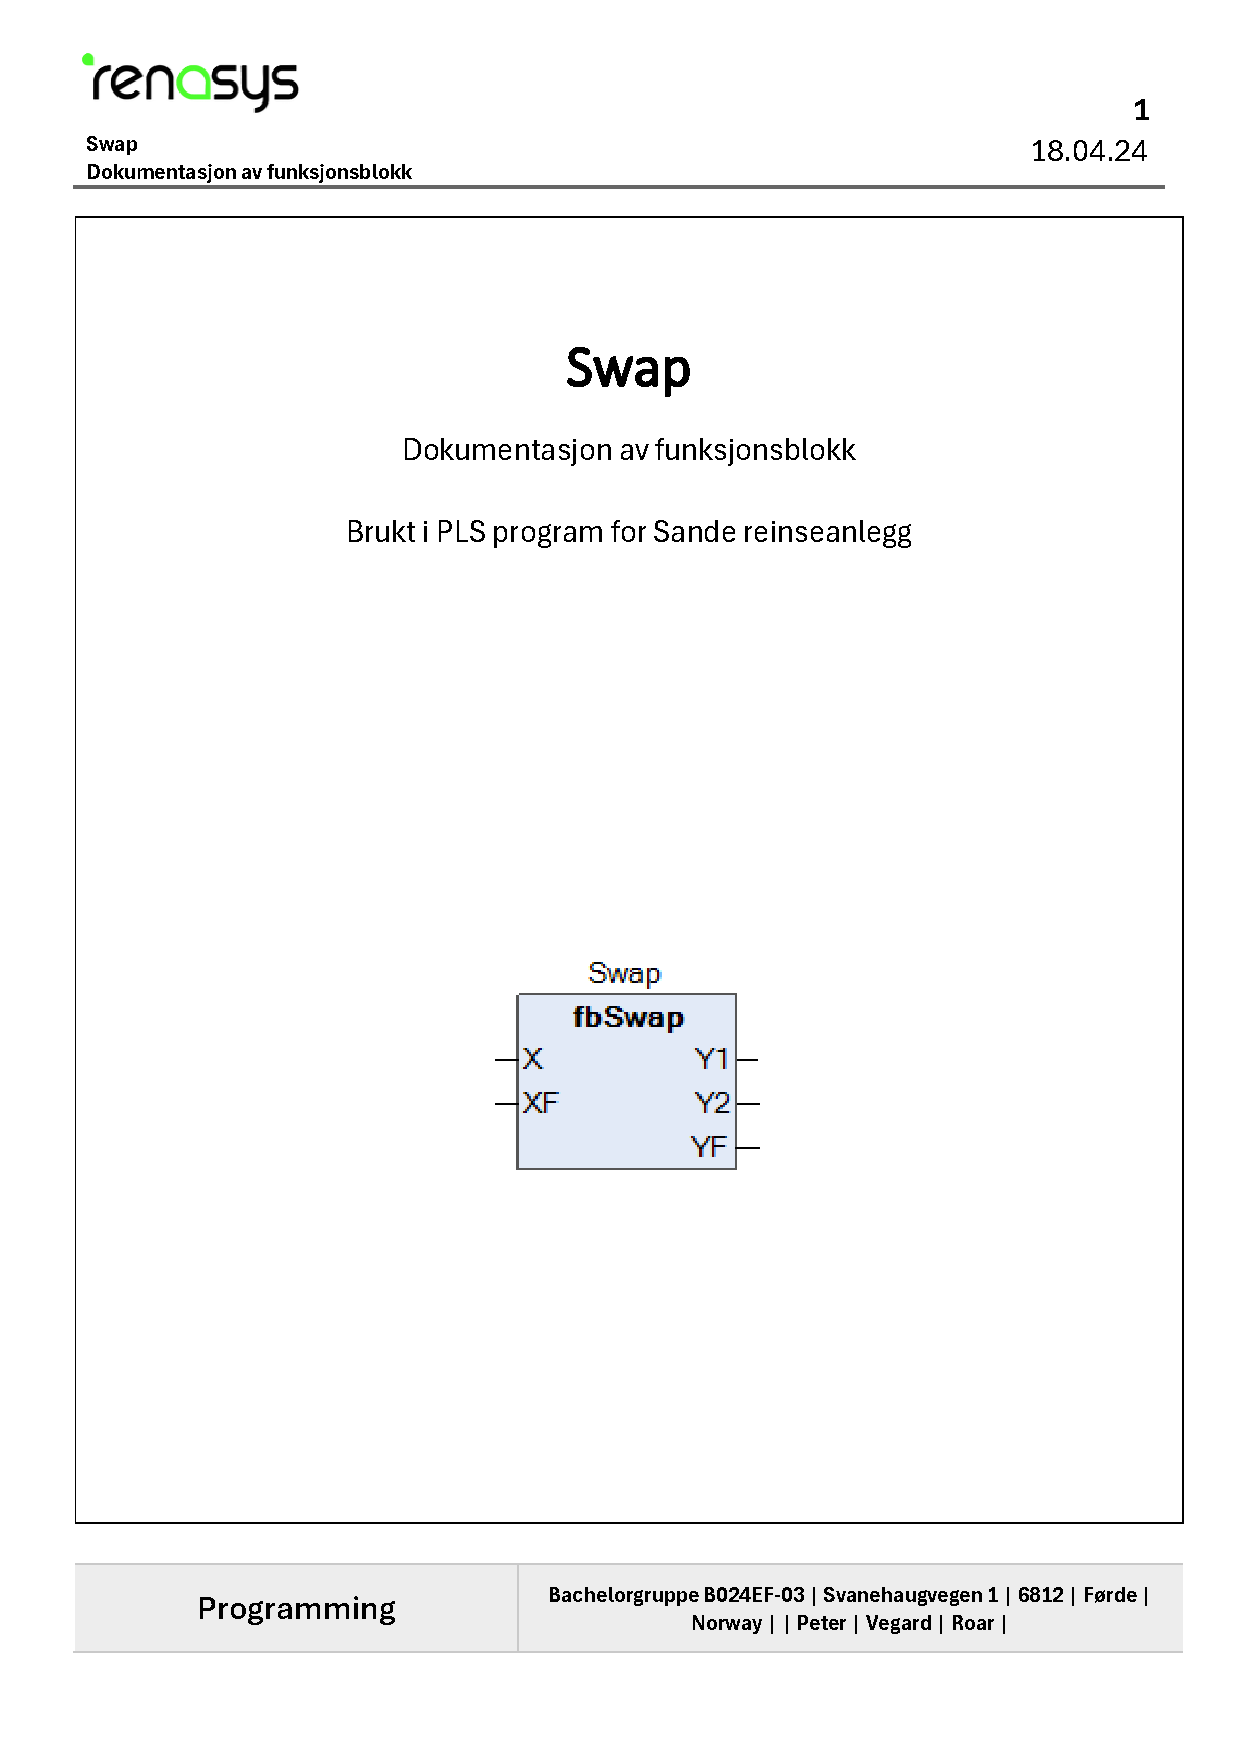
\includepdf[pages=1, scale=0.8, pagecommand={\section{FB Swap}\thispagestyle{fancy}}, fitpaper=true ]{Vedlegg/Funksjons Blokker/fbSwap Dokumentasjon.pdf}
\includepdf[pages=2-,scale=0.8, pagecommand={\thispagestyle{fancy}},fitpaper=true]{Vedlegg/Funksjons Blokker/fbSwap Dokumentasjon.pdf}
% Time Meter
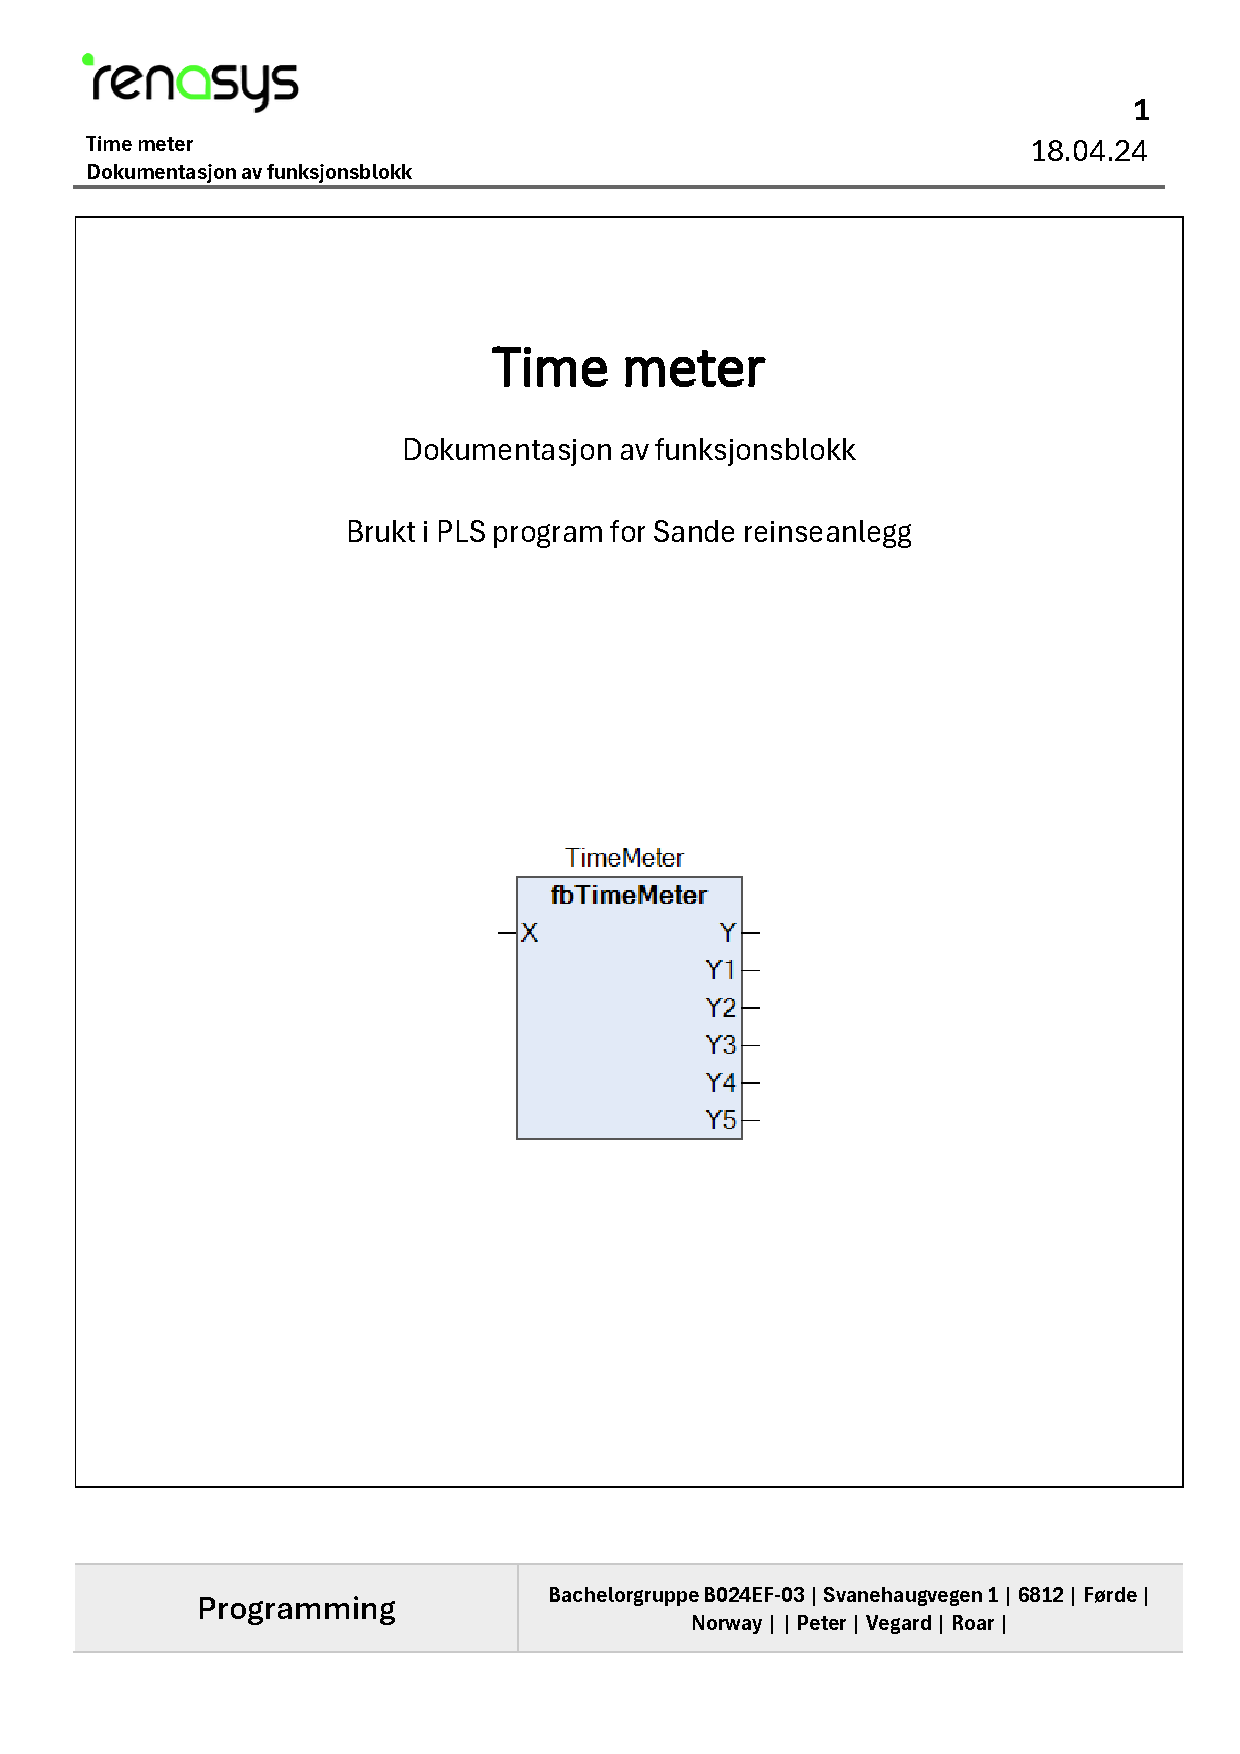
\includepdf[pages=1, scale=0.8, pagecommand={\section{FB Time Meter}\thispagestyle{fancy}}, fitpaper=true ]{Vedlegg/Funksjons Blokker/fbTimeMeter Dokumentasjon.pdf}
\includepdf[pages=2-,scale=0.8, pagecommand={\thispagestyle{fancy}},fitpaper=true]{Vedlegg/Funksjons Blokker/fbTimeMeter Dokumentasjon.pdf}
% Timer
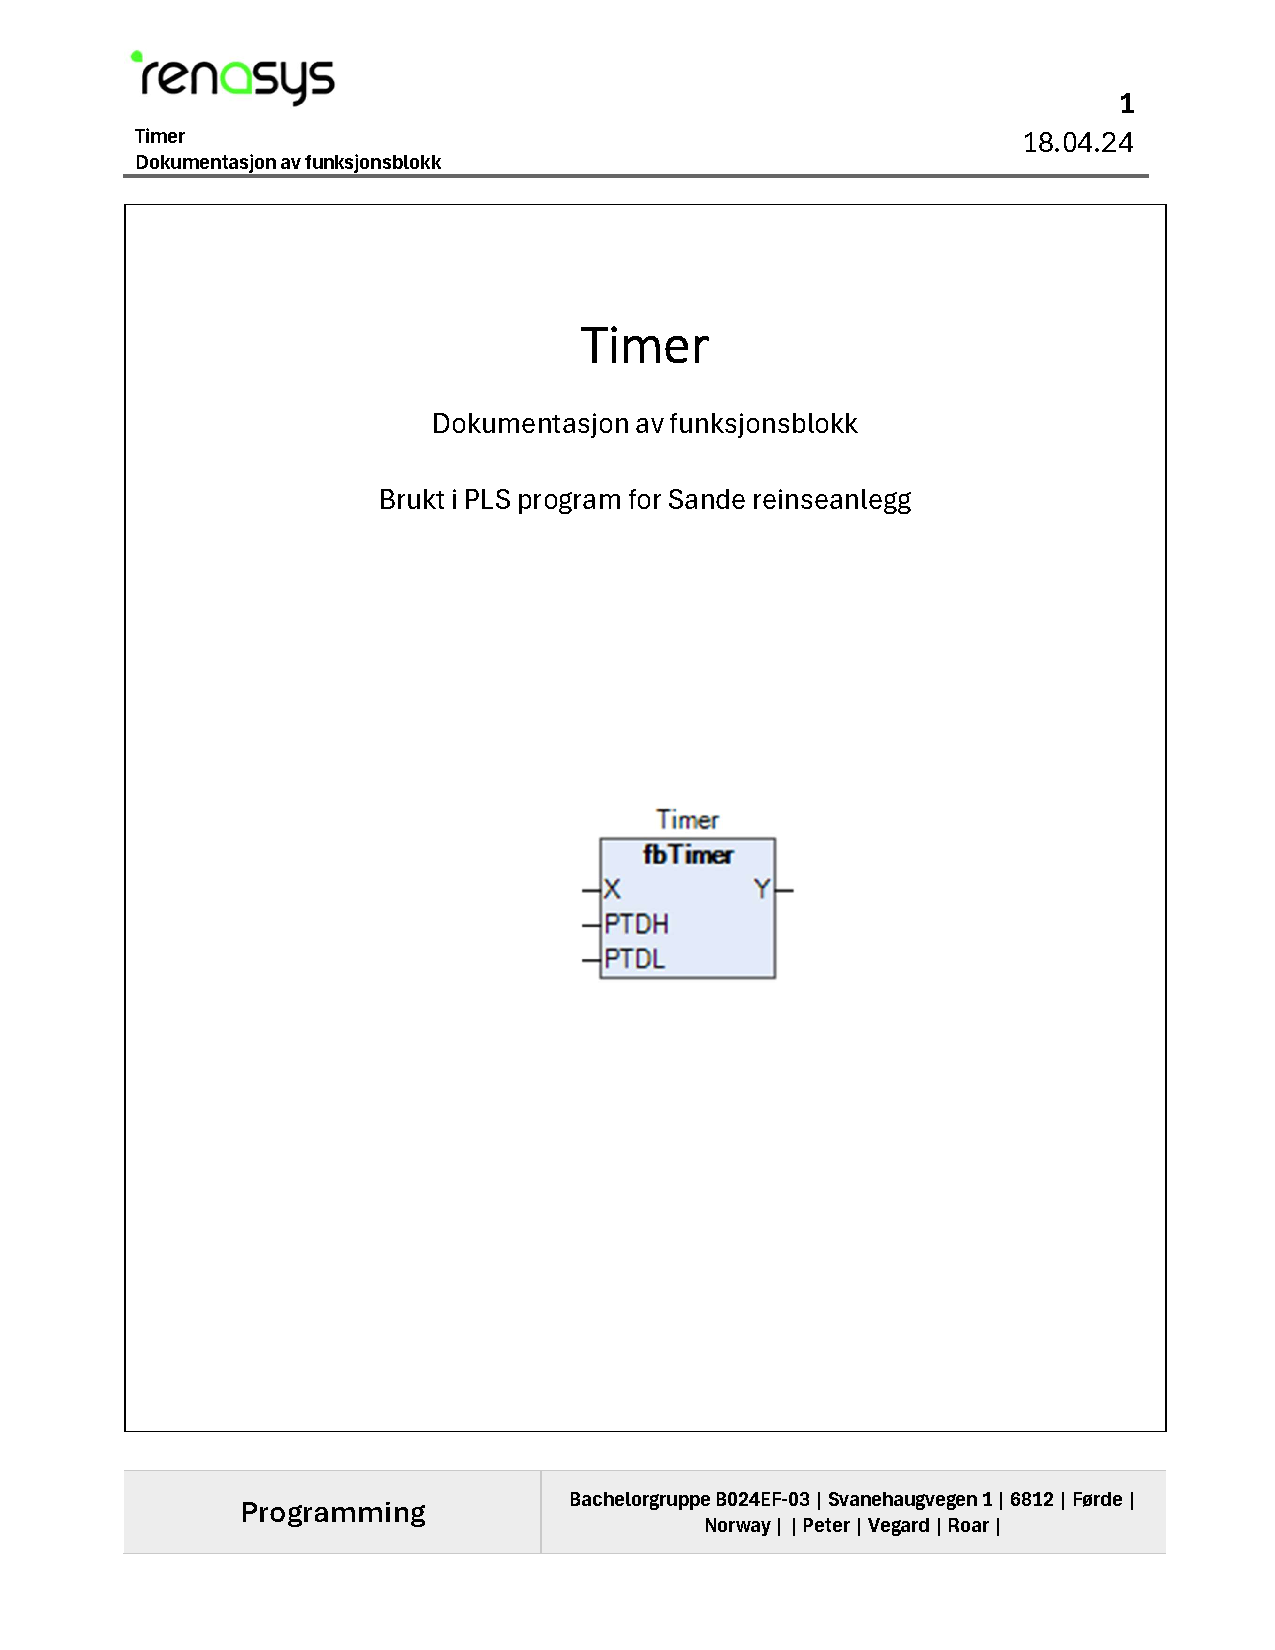
\includepdf[pages=1, scale=0.8, pagecommand={\section{FB Timer}\thispagestyle{fancy}}, fitpaper=true ]{Vedlegg/Funksjons Blokker/fbTimer.pdf}
\includepdf[pages=2-,scale=0.8, pagecommand={\thispagestyle{fancy}},fitpaper=true]{Vedlegg/Funksjons Blokker/fbTimer.pdf}


\chapter{IEC Blokker}
% MB Blokk
% Include only the first page
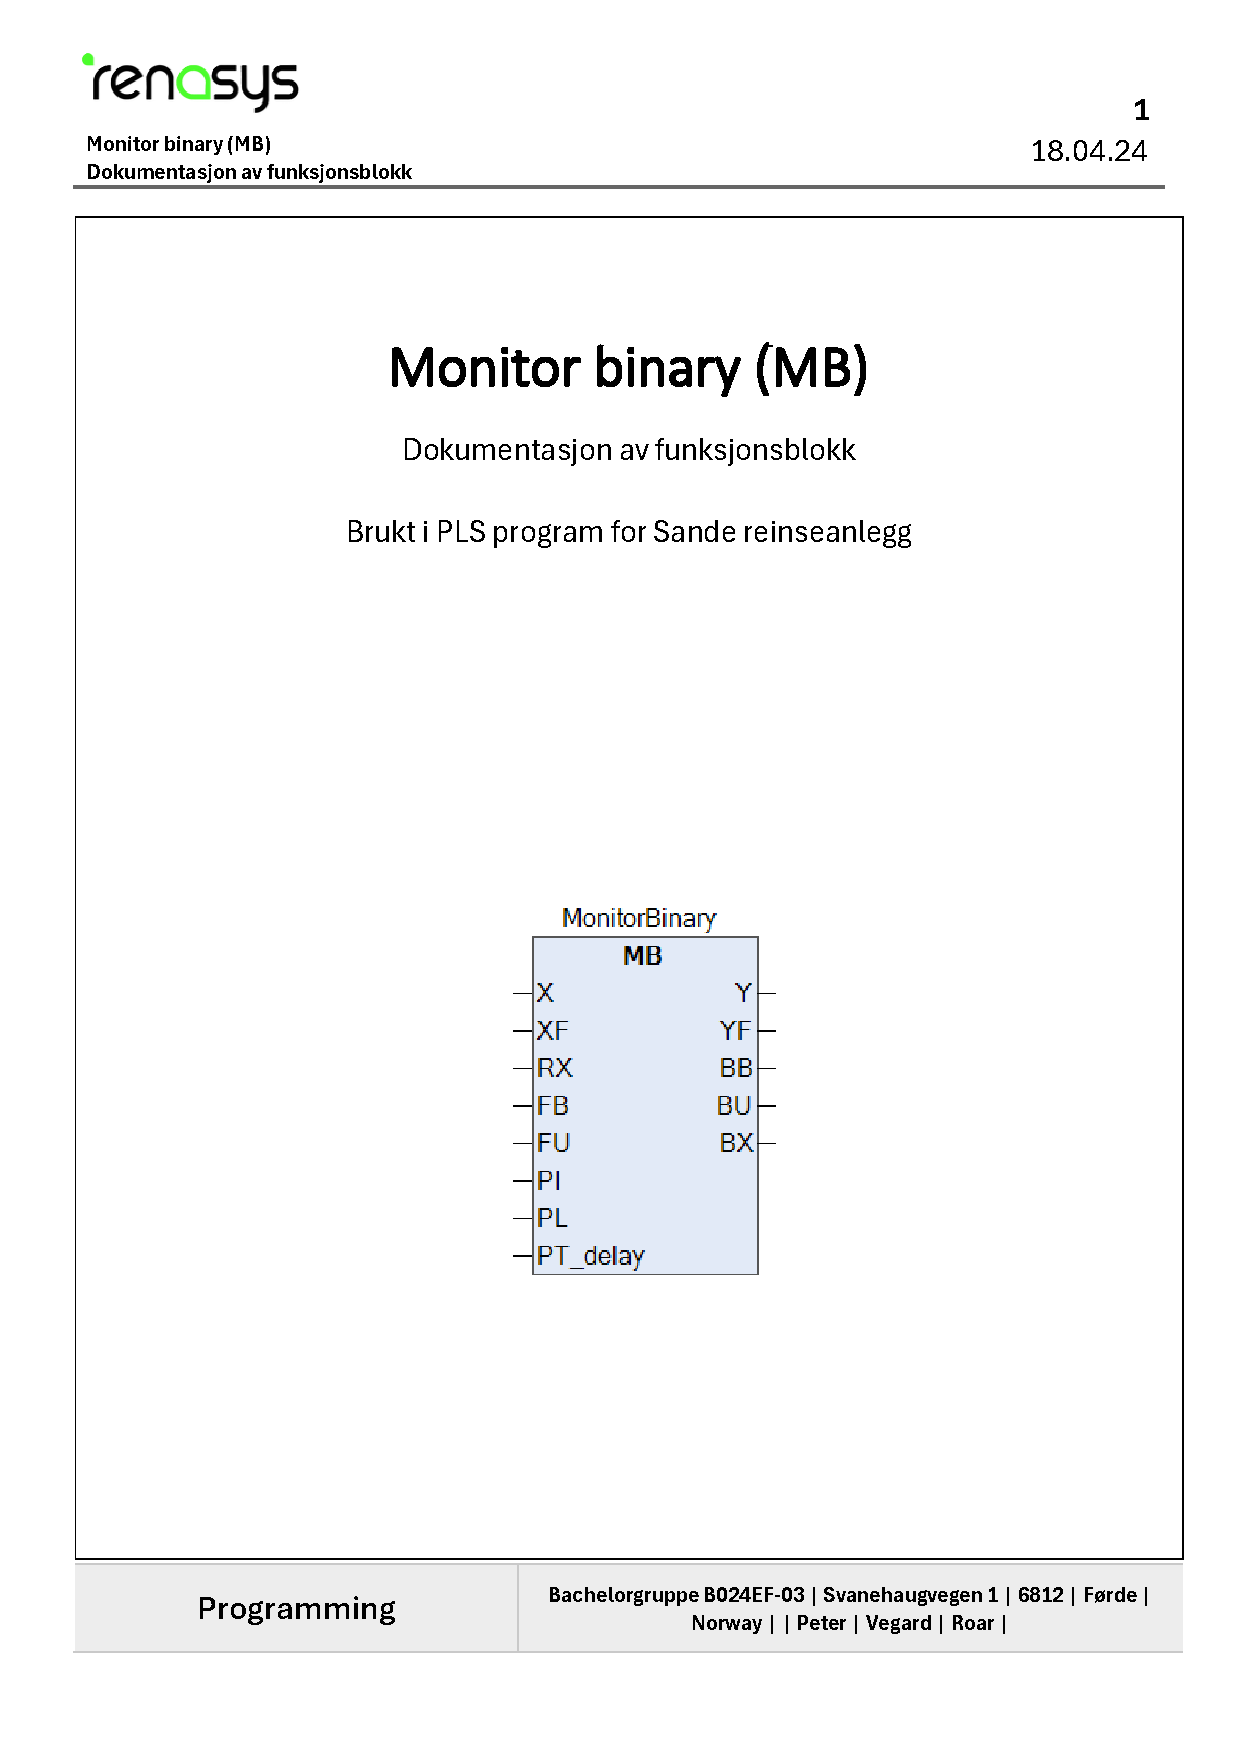
\includepdf[pages=1,scale=0.8, pagecommand={\section{Montor binary}\thispagestyle{fancy}},fitpaper=true]{Vedlegg/IEC Blokker/MB Dokumentasjon.pdf}
% Include the rest of the pages, Starts from the second page to the last, Keep the same scale for all pages
\includepdf[pages=2-, scale=0.8, pagecommand={\thispagestyle{fancy}}, fitpaper=true]{Vedlegg/IEC Blokker/MB Dokumentasjon.pdf}

% MA Blokk
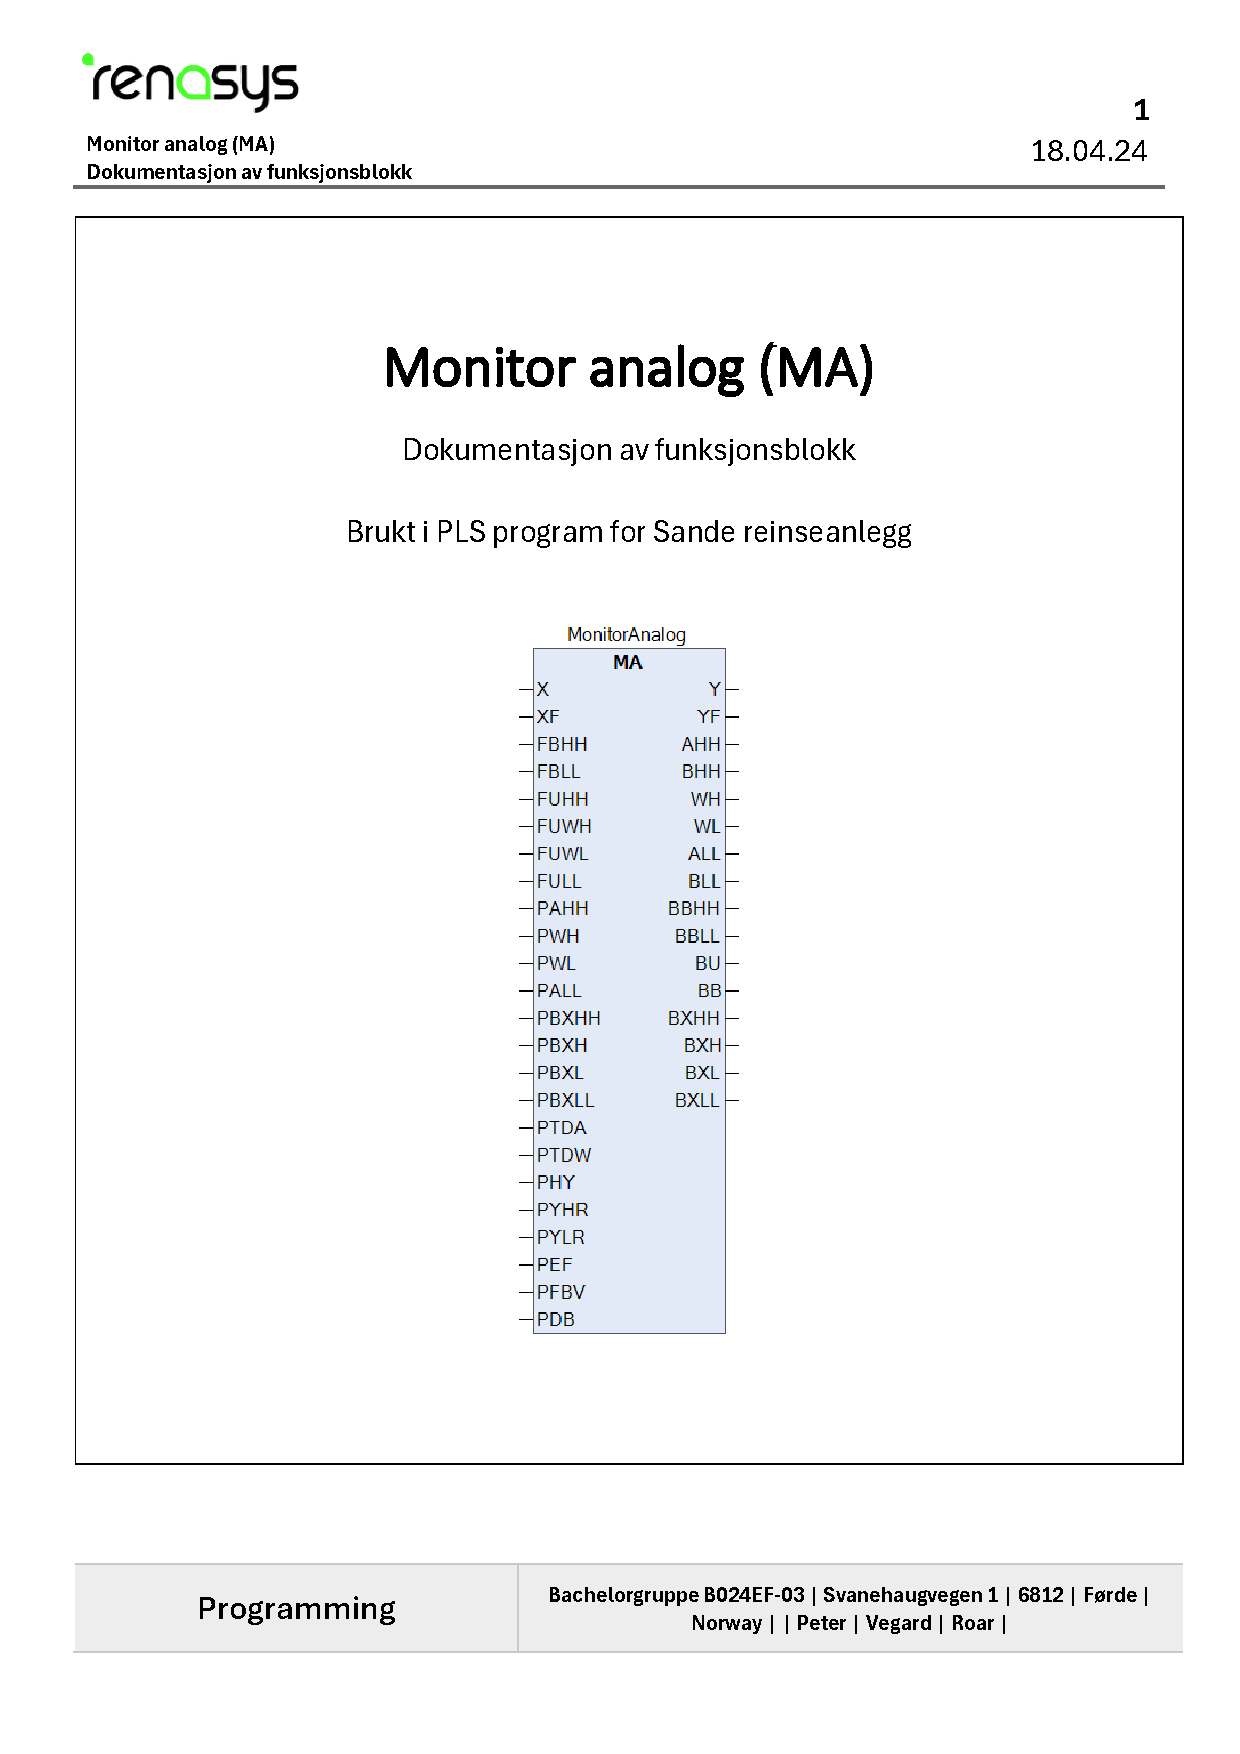
\includepdf[pages=1, scale=0.8, pagecommand={\section{Monitor Analogue}\thispagestyle{fancy}}, fitpaper=true ]{Vedlegg/IEC Blokker/MA Dokumentasjon.pdf}
\includepdf[pages=2-,scale=0.8, pagecommand={\thispagestyle{fancy}},fitpaper=true]{Vedlegg/IEC Blokker/MA Dokumentasjon.pdf}

% SBE Blokk
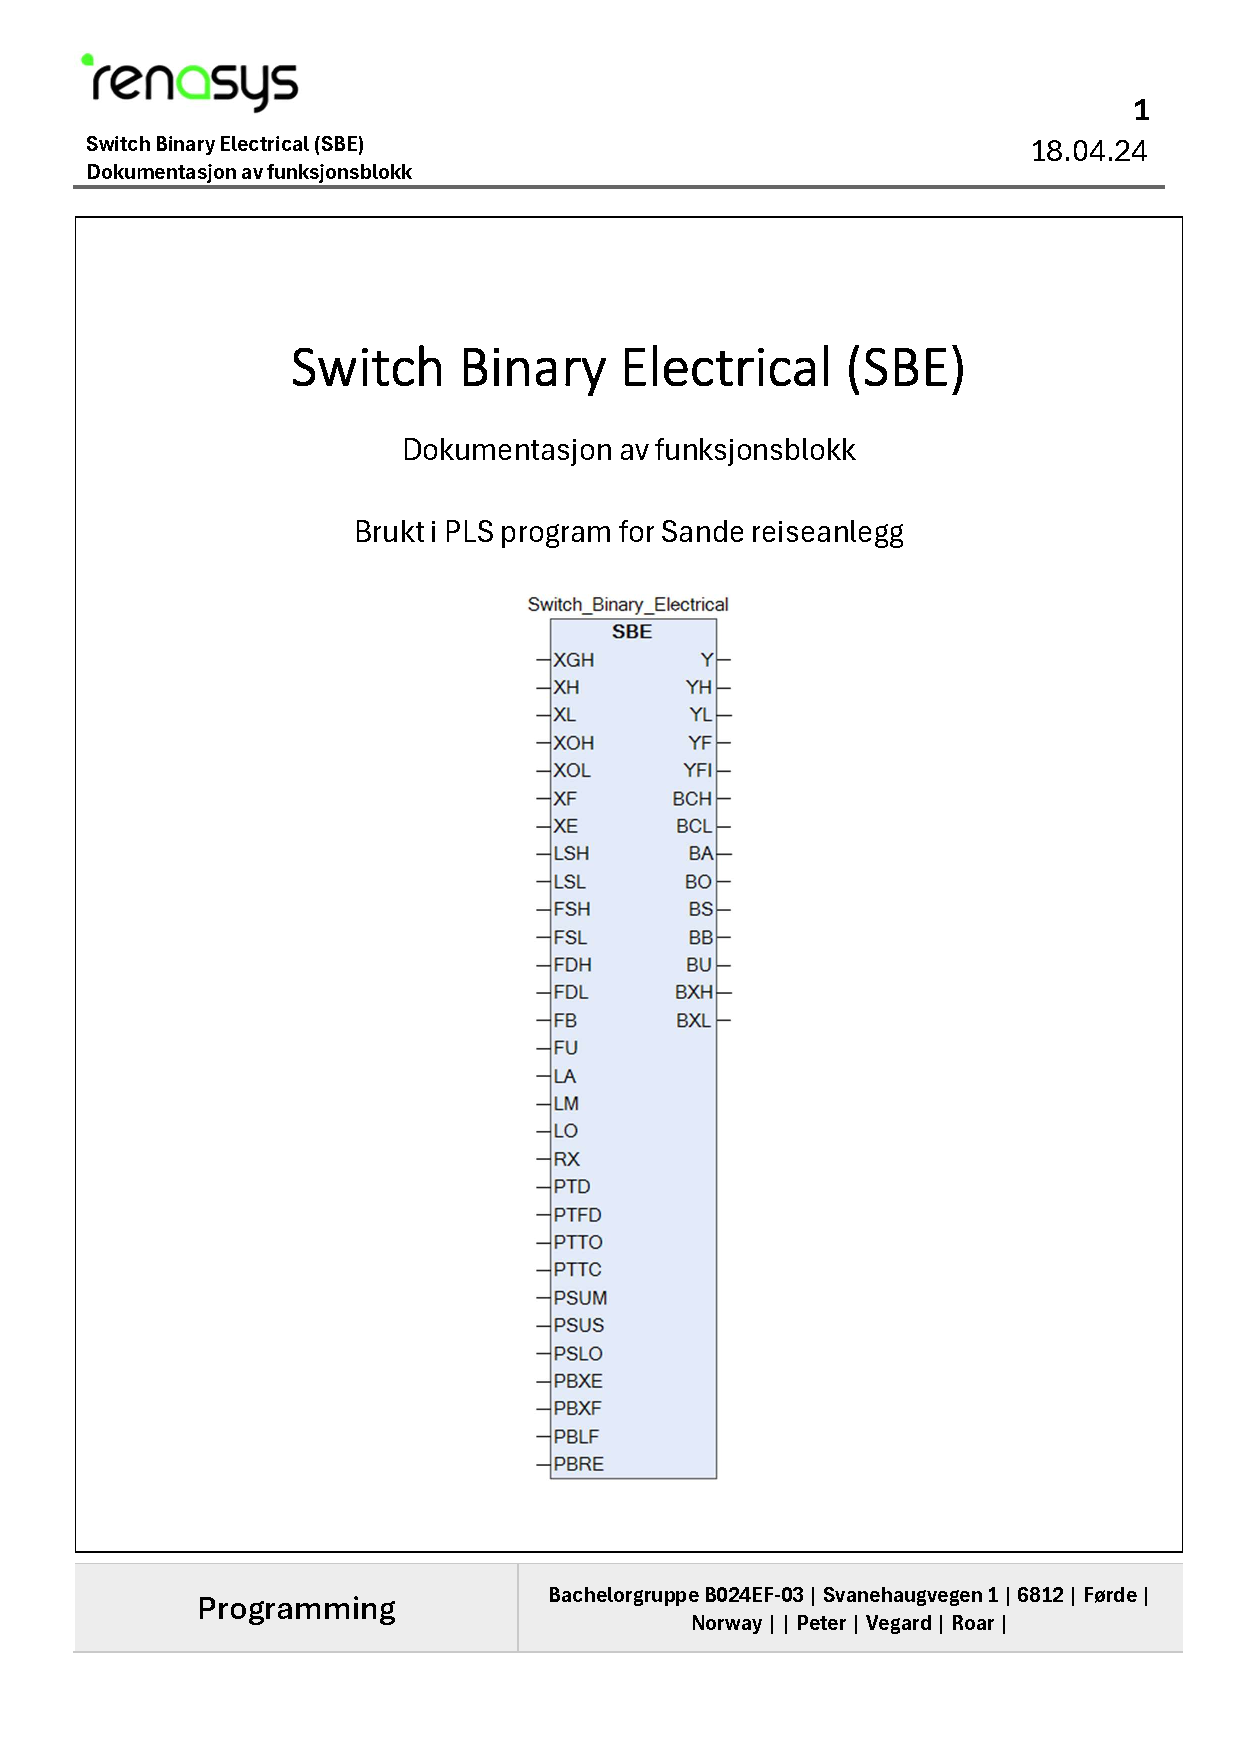
\includepdf[pages=1, scale=0.8, pagecommand={\section{Switch Binary Eletrical}\thispagestyle{fancy}}, fitpaper=true ]{Vedlegg/IEC Blokker/SBE Dokumentasjon.pdf}
\includepdf[pages=2-,scale=0.8, pagecommand={\thispagestyle{fancy}},fitpaper=true]{Vedlegg/IEC Blokker/SBE Dokumentasjon.pdf}

% SBV Blokk
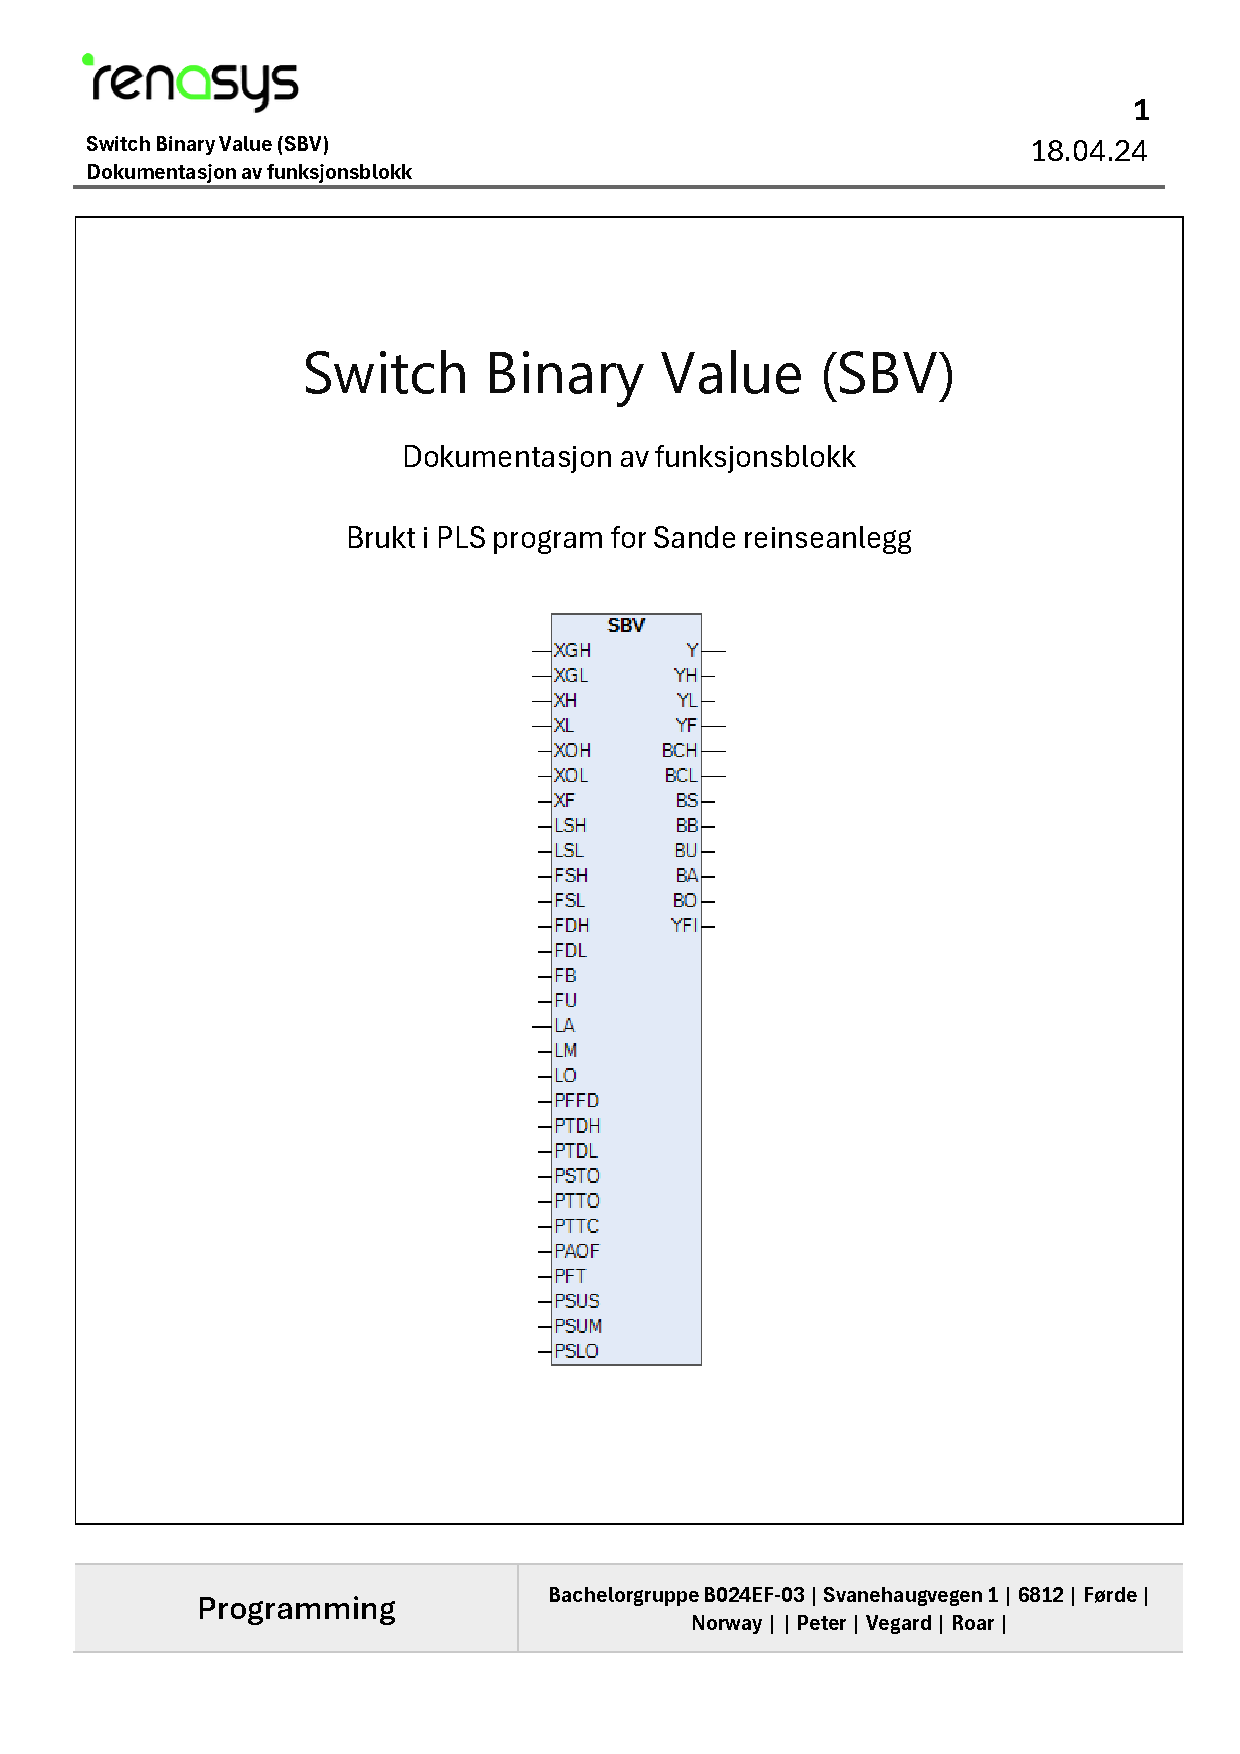
\includepdf[pages=1, scale=0.8, pagecommand={\section{Switch Binary Valve}\thispagestyle{fancy}}, fitpaper=true ]{Vedlegg/IEC Blokker/SBV Dokumentasjon.pdf}
\includepdf[pages=2-,scale=0.8, pagecommand={\thispagestyle{fancy}},fitpaper=true]{Vedlegg/IEC Blokker/SBV Dokumentasjon.pdf}


% ----------- Nytt Kapittel
\chapter{Funksjoner}
% Volume Rektangel

\includepdf[pages=1, scale=0.8, pagecommand={\section{FC Volum rektangel}\thispagestyle{fancy}}, fitpaper=true ]{Vedlegg/Funksjoner/Volume_Rectangle.pdf}

\includepdf[pages=2-,scale=0.8, pagecommand={\thispagestyle{fancy}},fitpaper=true]{Vedlegg/Funksjoner/Volume_Rectangle.pdf}
% Volume Sylinder

\includepdf[pages=1, scale=0.8, pagecommand={\section{FC Volum Sylinder}\thispagestyle{fancy}}, fitpaper=true ]{Vedlegg/Funksjoner/Volume_Cylinder.pdf}

\includepdf[pages=2-,scale=0.8, pagecommand={\thispagestyle{fancy}},fitpaper=true]{Vedlegg/Funksjoner/Volume_Cylinder.pdf}

% ----------- Nytt Kapittel
\chapter{Alarmlister}

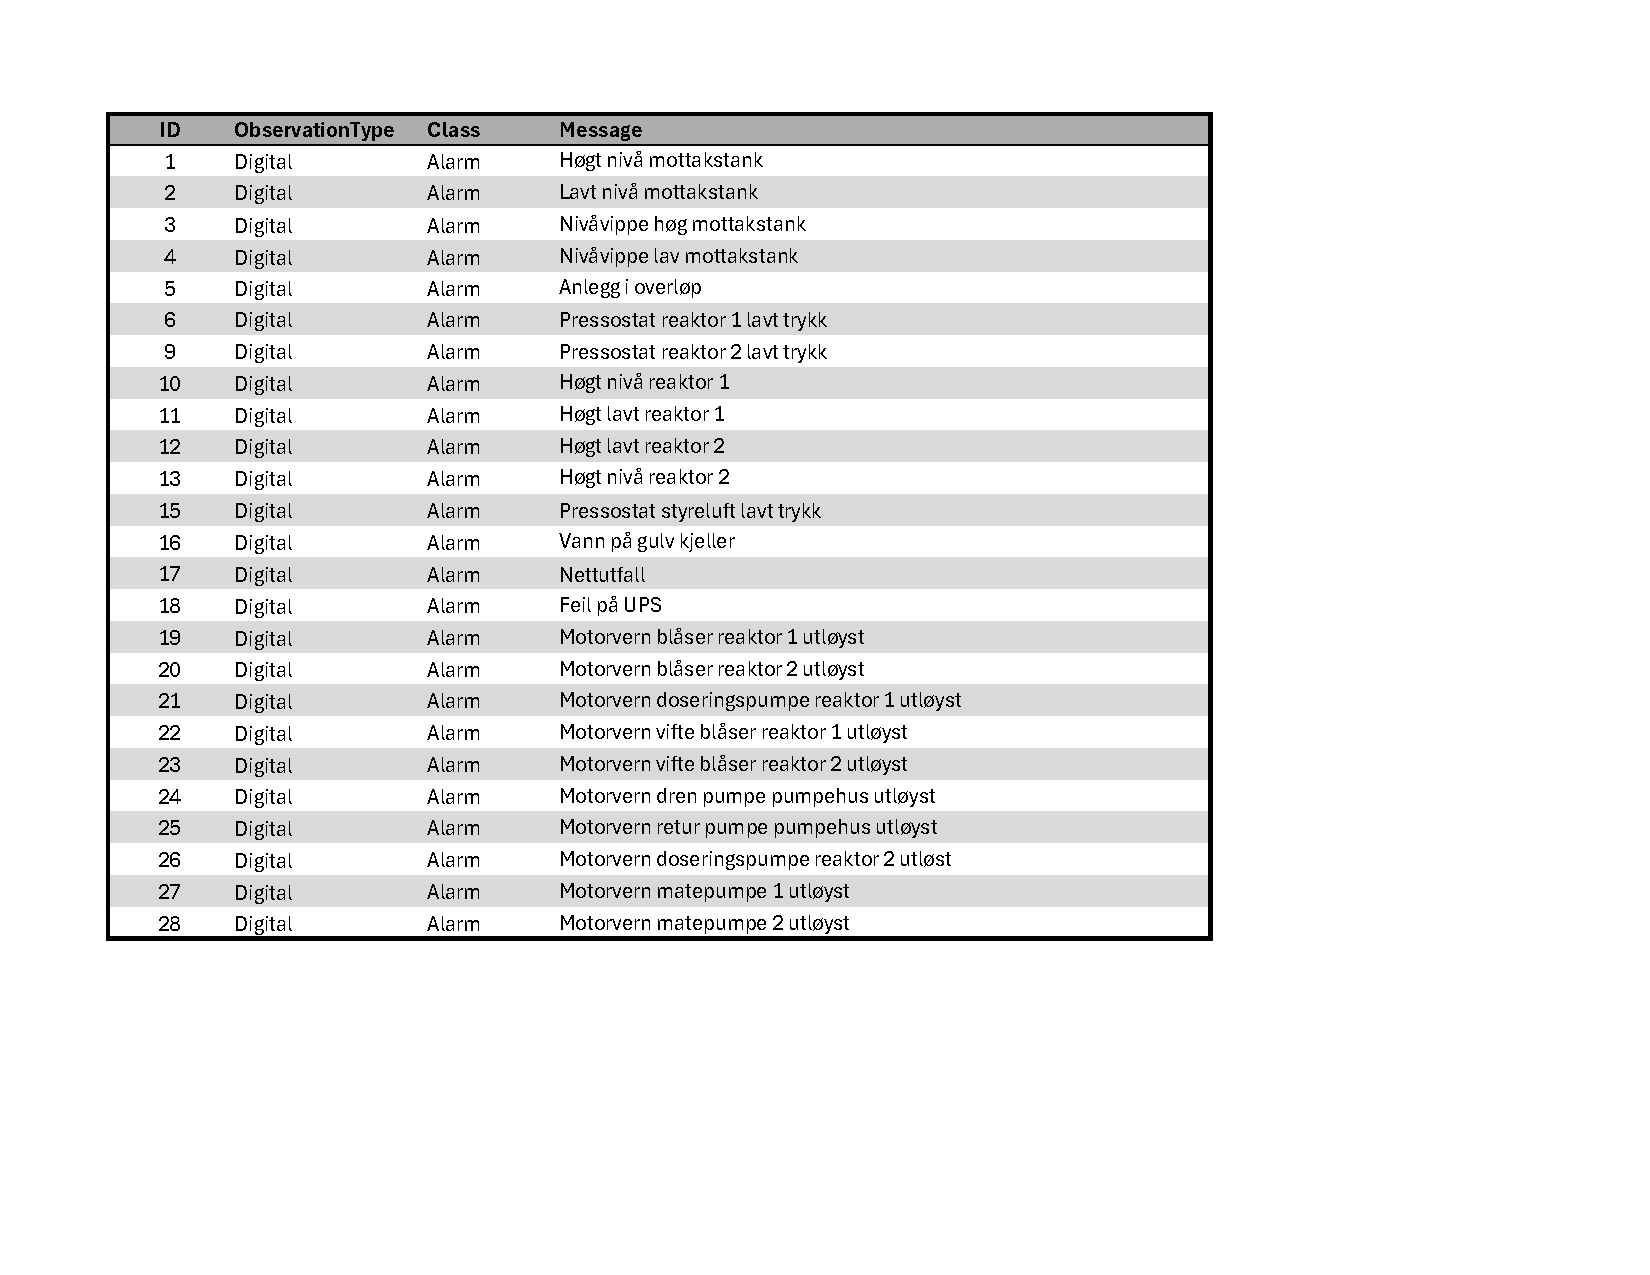
\includepdf[pages=1, scale=0.8, pagecommand={\section{Alarm liste}\thispagestyle{fancy}}, fitpaper=true ]{Vedlegg/AlarmLister/AlarmListe.pdf}

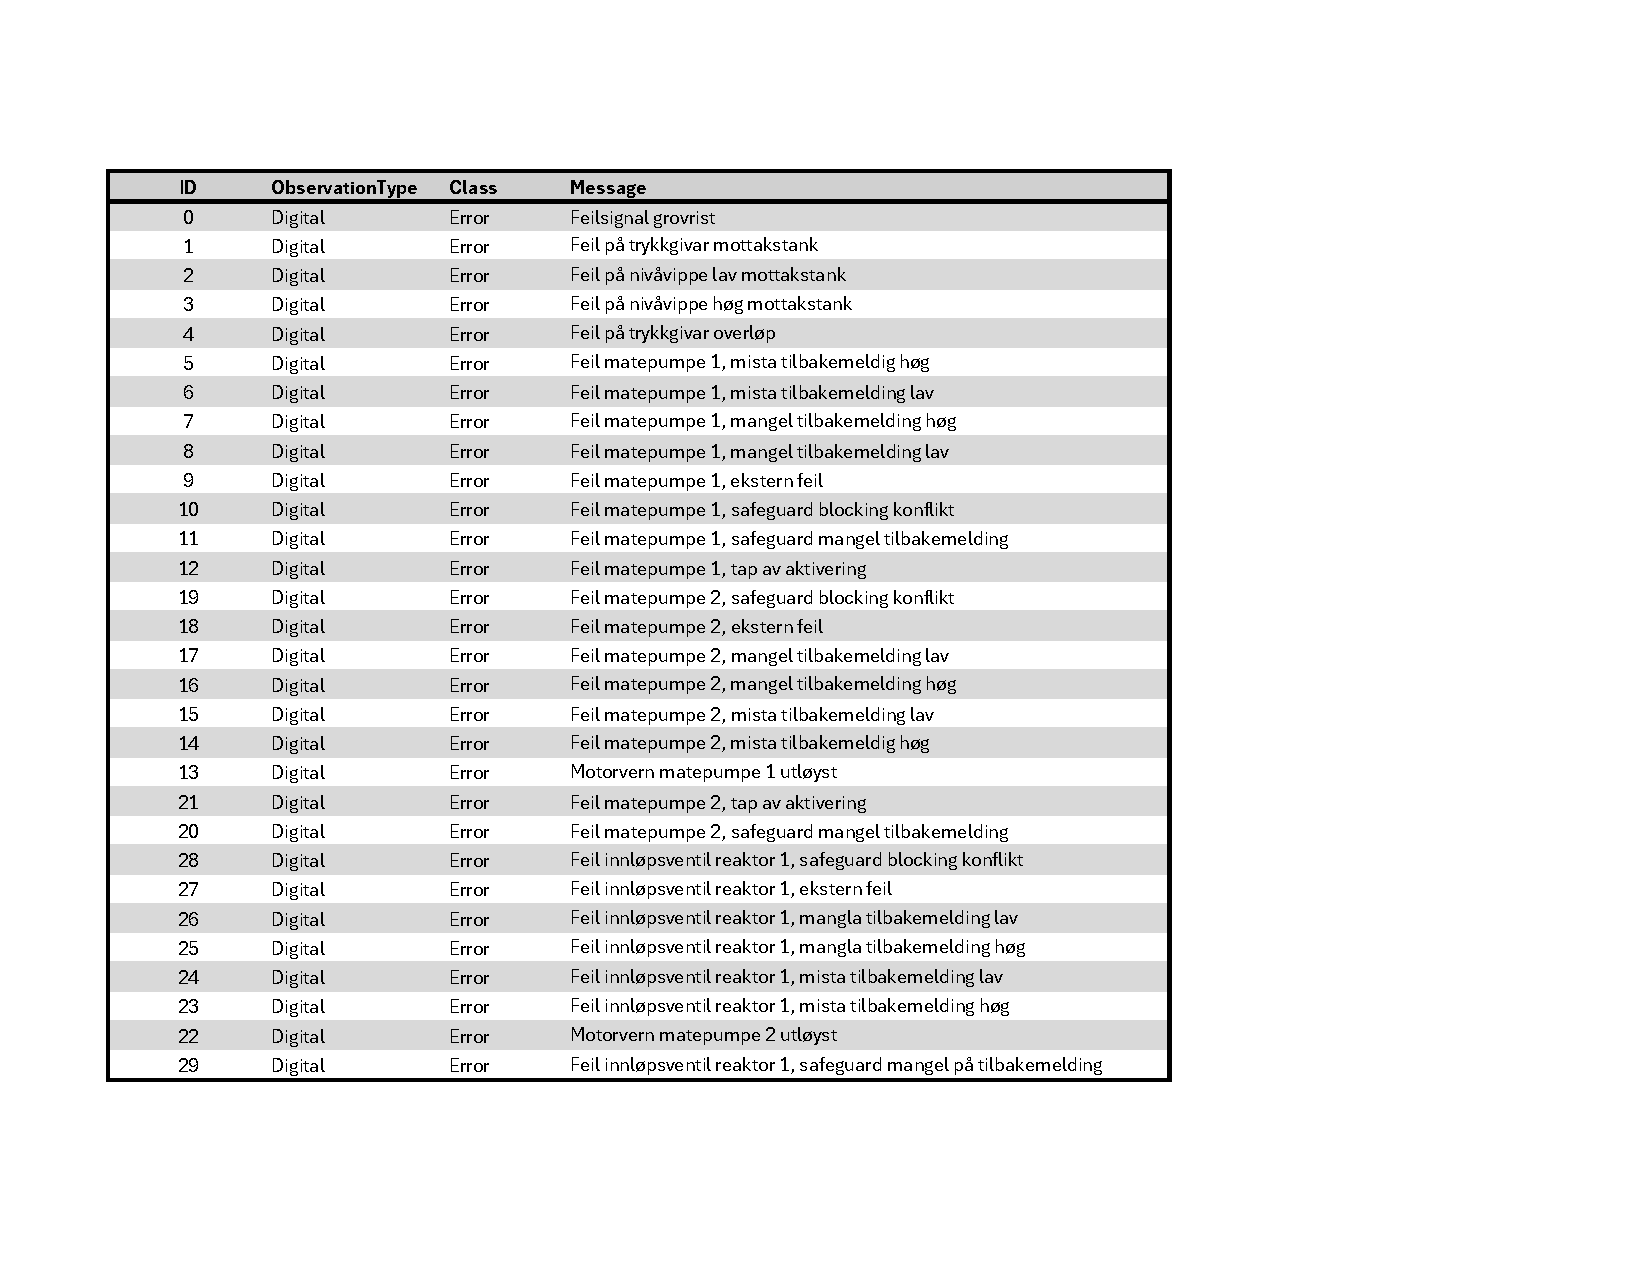
\includepdf[pages=1, scale=0.8, pagecommand={\section{Error liste}\thispagestyle{fancy}}, fitpaper=true ]{Vedlegg/AlarmLister/ErrorListe.pdf}
\includepdf[pages=2-,scale=0.8, pagecommand={\thispagestyle{fancy}},fitpaper=true]{Vedlegg/AlarmLister/ErrorListe.pdf}

% ----------- Nytt Kapittel
% Driftsinstruks Sande

\includepdf[pages=1, scale=0.8, pagecommand={\chapter{Driftsinstruks Orginal}\thispagestyle{fancy}}, fitpaper=true ]{Vedlegg/Driftsinstruks_Sande_RA_Orginal.pdf}
\includepdf[pages=2-,scale=0.8, pagecommand={\thispagestyle{fancy}},fitpaper=true]{Vedlegg/Driftsinstruks_Sande_RA_Orginal.pdf}

% ----------- Nytt Kapittel
% Funksjonsbeskrivelse Sande
\includepdf[pages=1, scale=0.8, pagecommand={\chapter{Funksjonsbeskrivelse}\thispagestyle{fancy}}, fitpaper=true ]{Vedlegg/Funksjonsbeskrivelse.pdf}
\includepdf[pages=2-,scale=0.8, pagecommand={\thispagestyle{fancy}},fitpaper=true]{Vedlegg/Funksjonsbeskrivelse.pdf}

% ----------- Nytt Kapittel
% SCD Diagrammer

{\raggedright
\chapter{Sekvensar}\par
}
%\includepdf[pages=1, angle=90, pagecommand={\section{Tilstand Pause}\thispagestyle{fancy}}, fitpaper=true]{Vedlegg/SCD.pdf}
%\includepdf[pages=2, angle=90, pagecommand={\section{Tilstand Innpumping}\thispagestyle{fancy}}, fitpaper=true]{Vedlegg/SCD.pdf}
%\includepdf[pages=3, angle=90, pagecommand={\section{Tilstand Reaksjon}\thispagestyle{fancy}}, fitpaper=true]{Vedlegg/SCD.pdf}
%\includepdf[pages=4, angle=90, pagecommand={\section{Tilstand Sedimentering}\thispagestyle{fancy}}, fitpaper=true]{Vedlegg/SCD.pdf}
%\includepdf[pages=5, angle=90, pagecommand={\section{Tilstand Uttapping}\thispagestyle{fancy}}, fitpaper=true]{Vedlegg/SCD.pdf}
%\includepdf[pages=6, angle=90, pagecommand={\section{Tilstand Felles Styring}\thispagestyle{fancy}}, fitpaper=true]{Vedlegg/SCD.pdf}

%\section{Tilstand Pause1}
\thispagestyle{plain}
{
\raggedright
\section{Tilstand Pause}\par
}
\thispagestyle{fancy}
%\leftalignedsection{Tilstand Pause}
\begin{adjustwidth}{-3cm}{-3cm}
\begin{tikzpicture}[remember picture, overlay]
    % Include the PDF page rotated, positioned at the center of the page
    % Gammel scale for alle SCD var scale=0.36 for fullpage scale
    \node[inner sep=0pt] at (current page.center) {
        \includegraphics[page=1,angle=90, scale=0.27, keepaspectratio, trim=-100 -100 -100 -100]{Vedlegg/SCD.pdf}
    };
\end{tikzpicture}
\end{adjustwidth}
\newpage
\section{Tilstand Innpumping}
\begin{tikzpicture}[remember picture, overlay]
    % Include the PDF page rotated, positioned at the center of the page
    \node[inner sep=0pt] at (current page.center) {
        \includegraphics[page=2,angle=90, scale=0.28, keepaspectratio]{Vedlegg/SCD.pdf}
    };
\end{tikzpicture}
\newpage
\section{Tilstand Reaksjon}
\begin{tikzpicture}[remember picture, overlay]
    % Include the PDF page rotated, positioned at the center of the page
    \node[inner sep=0pt] at (current page.center) {
        \includegraphics[page=3,angle=90, scale=0.28, keepaspectratio]{Vedlegg/SCD.pdf}
    };
\end{tikzpicture}
\newpage
\section{Tilstand Sedimentering}
\begin{tikzpicture}[remember picture, overlay]
    % Include the PDF page rotated, positioned at the center of the page
    \node[inner sep=0pt] at (current page.center) {
        \includegraphics[page=4,angle=90, scale=0.28, keepaspectratio]{Vedlegg/SCD.pdf}
    };
\end{tikzpicture}
\newpage
\section{Tilstand Uttapping}
\begin{tikzpicture}[remember picture, overlay]
    % Include the PDF page rotated, positioned at the center of the page
    \node[inner sep=0pt] at (current page.center) {
        \includegraphics[page=5,angle=90, scale=0.28, keepaspectratio]{Vedlegg/SCD.pdf}
    };
\end{tikzpicture}
\newpage
\section{Tilstand Felles Styring}
\begin{tikzpicture}[remember picture, overlay]
    % Include the PDF page rotated, positioned at the center of the page
    \node[inner sep=0pt] at (current page.center) {
        \includegraphics[page=6,angle=90, scale=0.28, keepaspectratio]{Vedlegg/SCD.pdf}
    };
\end{tikzpicture}

% ----------- Nytt Kapittel
\chapter{Komponent liste}

% ----------- Nytt Kapittel
\chapter{IO liste}

\includepdf[pages=1, scale=0.8, pagecommand={\section{Alarm liste}\thispagestyle{fancy}}, fitpaper=true ]{Vedlegg/IOliste.pdf}